\documentclass[journal]{IEEEtran}
\usepackage[utf8]{inputenc}
\usepackage[T1]{fontenc}
\usepackage[spanish]{babel}
\usepackage{graphicx}
\usepackage{url}
\usepackage{hyperref}
\usepackage{float}
\hyphenation{op-tical net-works semi-conduc-tor}

\begin{document}

% paper title
\title{Dirección Efectiva en la Ingeniería de Sistemas Informáticos: Un Análisis de la Inteligencia Emocional y las Técnicas de Relaciones Humanas}

\author{Elmer Edenilson Rosales Molina,\\ ~\IEEEmembership{rm20001@ues.edu.sv;}\\
        Julio Cesar Mejía Rodriguez,\\ ~\IEEEmembership{mr20084@ues.edu.sv}}

\maketitle

\begin{abstract}
Esta investigación se dedica al estudio de la inteligencia emocional y las relaciones interpersonales en la dirección de la Ingeniería de Sistemas Informáticos. Se extrae habilidades selectivas de varios autores (Dale Carnegie \& Daniel Goleman) para adaptarlas en este campo. 
\end{abstract}

\begin{keywords}
IEEE, \LaTeX, inteligencia emocional, relaciones interpersonales, comunicación, empatía, autocontrol, motivación, dirección.
\end{keywords}

\IEEEpeerreviewmaketitle

\section{Introducción}
Muchas veces pensamos que las personas con las mejores notas o con mucha preparación profesional son los mejores candidatos para el desempeño de puestos de liderazgo en las empresas u organizaciones, pero un aspecto esencial que casi nunca es tomado en cuenta, es la capacidad de inteligencia emocional que los individuos poseen, este tipo de inteligencia abarca 5 habilidades, que según Goleman son susceptibles de aprenderse y perfeccionase a lo largo de la vida, si para ello se utilizan los métodos adecuados.

Estas habilidades son: Autocontrol, Entusiasmo, Empatía, Perseverancia y Automotivación. El diseño biológico que rige nuestras emociones constituye un impulso que nos moviliza a la acción, es por ellos que el mismo significado de la palabra en latín “moveré” significa moverse y el prefijo e denota un objetivo. La emoción, entonces, desde el plano semántico, significa “movimiento hacia”, y basta con observar a los animales o a los niños pequeños para encontrar la forma en que las emociones los dirigen hacia una acción determinada, que puede ser huir, llora, etc.

Nuestra experiencia en la vida y el medio en el cual hayamos vivido moldean nuestras respuestas ante los estímulos emocionales que encontramos.

Alrededor del tallo encefálico, que constituye la región más primitiva de nuestro cerebro y que regula las funciones básicas como la respiración o el metabolismo, se fue configurando el sistema límbico, que aporta las emociones al repertorio de respuestas cerebrales. Gracias a éste, nuestros primeros ancestros pudieron ir ajustando sus acciones para adaptarse a las exigencias de un entorno cambiante. Así, fueron desarrollando la capacidad de identificar los peligros, temerlos y evitarlos. La evolución del sistema límbico estuvo, por tanto, aparejada al desarrollo de dos potentes herramientas: la memoria y el aprendizaje.

En esta región cerebral se ubica la amígdala, que tiene la forma de una almendra y que, de hecho, recibe su nombre del vocablo griego que denomina a esta última. Se trata de una estructura pequeña, aunque bastante grande en comparación con la de nuestros parientes evolutivos, en la que se depositan nuestros recuerdos emocionales y que, por ello mismo, nos permite otorgarle significado a la vida. Sin ella, nos resultaría imposible reconocer las cosas que ya hemos visto y atribuirles algún valor.

Sobre esta base cerebral en la que se asientan las emociones, fue creándose hace unos cien millones de años el neocórtex: la región cerebral que nos diferencia de todas las demás especies y en la que reposa todo lo característicamente humano. El pensamiento, la reflexión sobre los sentimientos, la comprensión de símbolos, el arte, la cultura y la civilización encuentran su origen en este esponjoso reducto de tejidos neuronales.

A parte, existe una habilidad inherente en los seres humanos para interactuar con los demás. Un forma eficaz para lograr el éxito en la vida y despertar el entusiasmo entre las personas son las habilidades para interactuar. Los seres humanos somos sociales y diariamente necesitamos la ayuda de otros, usualmente, en la desarrollo de proyectos de TI es indispensable manejar una buena comunicación entre los participantes para obtener el éxito del mismo. En este caso Dale Carnegie en su libro “Cómo ganar amigos e influir sobre las personas” presenta diversas técnicas que pueden ayudar a mejorar las relaciones interpersonales en todos los ambitos de la vida. 

Expresa las formas en las que se puede aplicar estas técnicas con naturalidad y fomentar ambientes de trabajo más agradables para mejorar la productividad y la motivación de las personas. Cabe señalar que los proyectos informáticos son muy complejos y participan conocimientos multidisciplinarios, ahora bien, el líder debe dirigir con mucho cuidado estas relaciones para lograr el éxito. Por esta razón, la presente investigación muestra algunas técnicas relevantes para mantener una dirección efectiva en la Ingeniería de Sistemas Informáticos de acuerdo a la inteligencia emocional y las relaciones interpersonales que debe considerarse para lograr el éxito en cada proyecto. Se toman estas técnicas y se aplican a escenas particulares de este campo para brindar un panorama comprensible y conciso que favorece la dirección.

\hfill Febrero 02, 2024

\section{Objetivos}

\subsection{Objetivo general}
Evaluar y fortalecer la dirección efectiva en la Ingeniería de Sistemas Informáticos mediante el análisis de la inteligencia emocional y las técnicas de relaciones humanas.

\subsection{Objetivos específicos}
\begin{itemize}
	\item Explorar el grado de conciencia emocional que tienen los estudiantes de ingeniería de sistemas informáticos de la Facultad de Ingeniería y Arquitectura de la Universidad De El Salvador, Cede Central.
	\item Indagar sobre la percepción de los estudiantes que cursan la carrera de Ingeniería de Sistemas Informáticos en la Universidad de El Salvador, acerca de la relevancia de la inteligencia emocional y las relaciones interpersonales en el desarrollo de habilidades profesionales y el éxito académico.
	\item Investigar cómo la inteligencia emocional y la buena comunicación influye en la capacidad de los estudiantes inscritos en la carrera de Ingeniería de Sistemas Informáticos en la Universidad De El Salvador para resolver problemas de manera efectiva y colaborativa en equipos de trabajo.
	\item Analizar los niveles de estrés percibidos por los estudiantes de Ingeniería de Sistemas informáticos de la Universidad De El Salvador y cómo la inteligencia emocional puede influir en su bienestar emocional y manejo del estrés.
\end{itemize}

\section{Alcances}
\begin{itemize}
	\item Aunque se realizarán esfuerzos para seleccionar una muestra representativa de estudiantes de la Facultad de Ingeniería y Arquitectura de la Universidad De El Salvador, Cede Central, la participación voluntaria podría introducir sesgos de autoselección.
	\item La medición de la inteligencia emocional y las relaciones interpersonales a través de una encuesta puede ser limitada en su capacidad para capturar todos los aspectos complejos y sutiles de estos conceptos.
	\item Nivel de conocimiento previo que puedan tener los estudiantes entorno al significado de inteligencia emocional y relaciones interpersonales. 
\end{itemize}
\section{Organización y Relaciones Interpersonales}
\PARstart{E}{n} el mundo de la dirección, especialmente en el campo de la Ingeniería de Sistemas Informáticos, la organización y las relaciones interpersonales asumen un papel crucial. Debido a que la organización hace referencia a cómo se estructuran y coordinan las actividades y los recursos dentro de una empresa (lo cual no es tarea fácil), por consiguiente, las relaciones interpersonales se refieren a cómo los miembros del equipo interactúan entre sí para obtener metas establecidas.

En su libro “Cómo ganar amigos e influir sobre las personas”, Dale Carnegie presenta varias técnicas que pueden mejorar las relaciones interpersonales en un entorno de trabajo. Por ejemplo, sugiere que mostrar un interés genuino en los demás y ser un buen oyente puede ayudar a construir relaciones más fuertes y más positivas. Estas técnicas pueden ser especialmente útiles en un entorno de TI, donde la colaboración y la comunicación efectiva son esenciales para el éxito del proyecto.

Además, Carnegie enfatiza la importancia de hacer que las personas se sientan importantes y valoradas. Esta técnica puede ser especialmente relevante para la organización en un entorno de TI. Al hacer que los miembros del equipo se sientan valorados, los líderes pueden aumentar la motivación y el compromiso del equipo, lo cual puede llevar a una mayor productividad y eficacia.

Por otro lado, en su libro “Inteligencia Emocional”, Daniel Goleman argumenta que la capacidad para reconocer, entender y gestionar nuestras emociones y las de los demás es crucial para las relaciones interpersonales. En un entorno de TI, donde los proyectos a menudo pueden ser estresantes y desafiantes, la inteligencia emocional puede ayudar a los líderes a manejar mejor el estrés y a resolver conflictos de manera efectiva.

%\begin{table}[H]
%% increase table row spacing, adjust to taste
%\renewcommand{\arraystretch}{1.3}
%\caption{An Example of a Table}
%\label{table_example}
%\centering
%\begin{tabular}{|c||c|}
%\hline
%One & Two\\
%\hline
%Three & Four\\
%\hline
%\end{tabular}
%\end{table}

\section{Dirección en el área de informática}
La dirección en el área de informática en las empresas es de vital importancia, ya que estas áreas son las encargadas de velar y administrar por la información crucial y esencial para el cumplimiento de las metas empresariales, es por ello que surge la necesidad de estudiar desde un punto psicoemocional el perfil de la/las personas destinadas a la administración y dirección del área de informática.

Este tópico adquiere una relevancia aún mayor cuando se considera el impacto de la inteligencia emocional en la gestión eficaz de estos departamentos. En su libro "Inteligencia Emocional", Daniel Goleman destaca cómo las habilidades emocionales son fundamentales para liderar equipos en cualquier contexto, y esto se aplica especialmente en el ámbito de la informática.

En un entorno altamente técnico y en constante evolución como es la informática, los líderes deben poseer una comprensión profunda tanto de la tecnología como de las personas que operan dentro de este campo. Es aquí donde entra en juego la inteligencia emocional, que se convierte en un elemento crucial para el éxito de la dirección en el área de informática.

Goleman señala que la inteligencia emocional abarca competencias como la autoconciencia ya que comprender las fortalezas, debilidades, valores y motivaciones personales y grupales permite tomar decisiones más informadas y efectivas. En el ámbito de TI, donde la toma de decisiones puede tener consecuencias significativas, la autoconciencia ayuda a evaluar objetivamente las situaciones y a liderar con claridad y determinación, otra es el autocontrol y la autogestión, estos son aspectos cruciales en el área de TI. En un entorno donde los plazos son ajustados y los desafíos son constantes, la capacidad de manejar el estrés, mantener la calma bajo presión y tomar decisiones racionales es esencial. Ya que la autogestión y autocontrol permite mantener el enfoque en los objetivos, superar los obstáculos y mantener la productividad incluso en las circunstancias más desafiantes, por otro lado, la empatía es también otra habilidad indispensable para la eficiente dirección de las áreas informáticas. Comprender las emociones y perspectivas de los miembros del equipo y de los superiores permite construir relaciones sólidas, fomentar un ambiente de trabajo positivo y promover la colaboración y el trabajo en equipo. Además, la empatía es una gran herramienta para abordar los conflictos de manera constructiva y también para motivar a nuestro equipo de manera efectiva hacia el logro de los objetivos comunes, y, por último, pero no menos importante se tienen a las habilidades sociales, estas desempeñan un papel crucial en el éxito de los líderes informáticos. La capacidad de comunicarse claramente, escuchar activamente y proporcionar retroalimentación constructiva es fundamental para dirigir un equipo de manera efectiva. Ya que las habilidades sociales permiten inspirar confianza, fomentar la creatividad y construir relaciones sólidas tanto dentro como fuera del equipo, lo que es esencial en un campo tan colaborativo como el de la informática.

La dirección en el área de informática va más allá de simplemente gestionar tecnología y datos; implica también entender y guiar a las personas que conforman estos equipos. La inteligencia emocional, tal como describe Goleman, emerge como un componente esencial en este proceso. Desde la autoconciencia hasta las habilidades sociales, cada aspecto de la inteligencia emocional expresada por Goleman se convierte en una herramienta poderosa para los líderes informáticos en la búsqueda del éxito organizacional. Al integrar estos principios en la dirección de áreas de TI, las empresas pueden cultivar entornos de trabajo más colaborativos, productivos y adaptativos, impulsando así su competitividad en un mundo empresarial cada vez más digitalizado y dinámico.

\section{Comunicación Efectiva en la Dirección de Proyectos de TI}
La comunicación efectiva se considera una habilidad esencial para el éxito de cualquier proyecto, debido a que todos los participantes muestran lo mejor de sí mismos y actuan con sinergia en todas las actvidades del proyecto al crear un clima de trabajo agradable. 

Al hacer referencia en el campo de la Ingeniería de Sistemas Informáticos los proyectos de TI suelen ser complejos y requieren de un equipo compuesto por individuos con diferentes habilidades y conocimientos. Usualmente estos son multidisciplinarios y dinámicos, se necesita interactuar constantemente con diferentes actores.

Según Chavez, “Una buena comunicación permite establecer objetivos claros, alinear expectativas, resolver conflictos, compartir información, obtener feedback, generar confianza y fomentar la colaboración. Todo esto contribuye a mejorar la calidad, la eficiencia y la satisfacción de los proyectos de TI”.

\subsection{Aspectos que deben considerarse en cada proyecto}
En proyectos informáticos, la calidad del producto se debe múltiples factores que pueden ser cumplidos al trabajar en conjunto y de forma coordinada, por esta razón, el dirigente del proyecto debe considerar los siguientes puntos:
\begin{itemize}
	\item Definir el propósito y el alcance del proyecto, así como los roles y responsabilidades de cada participante.
	\item Utilizar los canales y herramientas adecuados para cada tipo de comunicación, ya sea oral, escrita, sincrónica o asincrónica.
	\item Ser claro, conciso, coherente y cortés en tus mensajes, evitando ambigüedades, jergas y tecnicismos innecesarios.
	\item Escuchar activamente a los demás, mostrando empatía, respeto y apertura.
	\item Solicitar y ofrece feedback constructivo, reconociendo los logros y las oportunidades de mejora.
	\item Mantener una comunicación fluida y frecuente, informando sobre el estado, los avances y los problemas del proyecto.
	\item Fomentar la participación y la colaboración de todos los involucrados, creando un ambiente de confianza y transparencia.
\end{itemize}

\subsection{El enfoque de Carnegie para mejorar la comunicación}
Dale Carnegie en su libro “Cómo ganar amigos e influir sobre las personas” proporciona técnicas para interactuar eficazmente con las personas lo cual contribuye a la buena comunicación entre los miembros del equipo. Por lo tanto, se citarán algunas de estas tecnicas:

\subsubsection{No critique, no condene ni se queje}
Según Carnegie, “La crítica es inútil porque pone a la otra persona en la defensiva, y por lo común hace que trate de justificarse. La crítica es peligrosa porque lastima el orgullo, tan precioso de la persona, hiere su sentido de la importancia y despierta su resentimiento.”

Ahora bien, de acuerdo a lo expuesto por este autor es posible que el líder de un proyecto se sienta tentado ha actuar con esa conducta lo cual no ayudaría en mucho. Si se analiza detenidamente en escenas de trabajo, podemos obtener lo siguiente:

\begin{itemize}
	\item \textbf{No critique:} En la dirección de proyectos de TI, es común encontrar errores y problemas. Sin embargo, criticar a los miembros del equipo por sus errores puede crear un ambiente de trabajo negativo y disminuir la moral del equipo. En lugar de criticar, un líder efectivo proporciona retroalimentación constructiva y ayuda a los miembros del equipo a aprender de sus errores.
	\item \textbf{No condene:} Condenar a los miembros del equipo por sus acciones puede crear resentimiento y conflictos dentro del equipo. Un líder efectivo se enfoca en resolver el problema en lugar de condenar a la persona. Esto puede incluir discutir el problema de manera abierta y honesta, buscar soluciones juntos y aprender de la experiencia.
	\item \textbf{No se queje: }Quejarse puede ser perjudicial para el ambiente de trabajo y puede disminuir la productividad del equipo. En lugar de quejarse, un líder efectivo se enfoca en encontrar soluciones a los problemas y mantener una actitud positiva.
\end{itemize}

Por lo expuesto anteriormente, metodologías agiles como SCRUM ofrecen espacios entre los miembros para exponer los avances realizados, además, cuando uno de ellos presenta dificultades para desempeñar su tarea todos los miembros del equipo unen su conocimiento y experiencia para solucionar el problema lo cual hace pensar la importancia de la comunicación.

\subsubsection{Demuestre aprecio honrado y sincero}
Se cita un viejo dicho, “Pasaré una sola vez por este camino; de modo que cualquier bien que pueda hacer o cualquier cortesía que pueda tener para con cualquier ser humano, que sea ahora. No la dejaré para mañana, ni la olvidaré, porque nunca más volveré a pasar por aquí.”

Según Carnegie, “Herir a la gente no sólo no la cambia, sino que es una tarea que nadie nos agradecerá”. En esta regla señala que el caracter humano posee una principio profundo que es el anhelo de ser apreciado, eso emmarca algo significativo en las personas y satisfacen sus deseos lo cual es muy diferente a la adulación porque genera sentido de importancia y mejora la calidad.

En ingeniería se puede reflexionar en la siguiente aplicación:
\begin{itemize}
	\item \textbf{Reconocimiento del trabajo bien hecho:} En la dirección de proyectos de TI, es importante reconocer y apreciar el trabajo bien hecho. Esto puede ser tan simple como agradecer a un miembro del equipo por su contribución o destacar el buen trabajo en una reunión de equipo. Este tipo de aprecio sincero puede aumentar la moral del equipo y motivar a los miembros del equipo a continuar haciendo un buen trabajo.
	\item \textbf{Valoración de las ideas y sugerencias:} Los líderes de proyectos de TI deben demostrar aprecio por las ideas y sugerencias de los miembros del equipo. Esto no solo fomenta un ambiente de innovación y creatividad, sino que también hace que los miembros del equipo se sientan valorados y respetados.
	\item \textbf{Apoyo durante los desafíos:} Los proyectos de TI a menudo pueden ser desafiantes y estresantes. Durante estos tiempos, demostrar aprecio por el esfuerzo y la dedicación de los miembros del equipo puede proporcionar un muy necesario impulso moral.
\end{itemize}

\subsubsection{Despierte en los demás un deseo vehemente}
En la dirección de proyectos de TI, es importante inspirar a los miembros del equipo a alcanzar sus metas y objetivos. Según Carnegie, “el único medio que se tiene para influir sobre la otra persona es hablar acerca de lo que se quiere y demostrarle cómo conseguirlo”. Esto puede implicar ayudar a los miembros del equipo a ver cómo su trabajo contribuye al éxito general del proyecto y cómo pueden crecer y desarrollarse profesionalmente.

Además, despertar un deseo vehemente en los demás también puede ser una poderosa herramienta de motivación. Carnegie argumenta que “quien puede hacer las cosas tiene al mundo entero consigo. Quien no puede, marcha solo por el camino”. En un entorno de TI, esto podría implicar motivar a los miembros del equipo a aprender nuevas habilidades, adoptar nuevas tecnologías o asumir nuevos desafíos.

Al despertar un deseo vehemente en los demás, los líderes de proyectos de TI pueden influir positivamente en sus equipos. Esto puede llevar a un mayor compromiso, una mayor productividad y, en última instancia, a un mayor éxito del proyecto.

\subsubsection{Seis maneras de agradar a los demás}
\begin{itemize}
	\item \textbf{Interésese sinceramente por los demás:} Carnegie sugiere mostrar un interés genuino en los demás. En la dirección de proyectos de TI, esto puede traducirse en prestar atención a las ideas y opiniones de los miembros del equipo, lo cual puede fomentar un ambiente de trabajo colaborativo y respetuoso.
	\item \textbf{Sonría:} Una actitud positiva puede ser contagiosa y puede ayudar a crear un ambiente de trabajo más agradable y productivo.
	\item \textbf{Recuerde que para toda persona su nombre es el sonido más dulce e importante en cualquier idioma:} Recordar y usar los nombres de los miembros del equipo puede demostrar respeto y aprecio, lo cual puede mejorar las relaciones interpersonales y la comunicación.
	\item \textbf{Sea un buen oyente. Anime a los demás a hablar de sí mismos:} Escuchar activamente a los miembros del equipo puede demostrar que valoras sus ideas y opiniones, lo cual puede fomentar una comunicación abierta y efectiva.
	\item \textbf{Hable en términos de los intereses de la otra persona:} Comprender y hablar en términos de los intereses de los miembros del equipo puede ayudar a motivarlos y a obtener su cooperación.
	\item \textbf{Haga que la otra persona se sienta importante y hágalo sinceramente:} Reconocer el valor y las contribuciones de los miembros del equipo puede aumentar su moral y su compromiso con el proyecto.
\end{itemize}

\section{Gestión de Conflictos en Proyectos Informáticos}
En la gestión de proyectos, especialmente en entornos dinámicos y colaborativos como el de TI los conflictos son inevitables. Estos pueden surgir debido a diferencias de opiniones, objetivos divergentes o simplemente por la naturaleza compleja y multifacética de los proyectos. Es por esto que entre las habilidades que destaca Goleman en su libro de inteligencia emocional, la empatía que proviene del griego empatheia (sentir dentro), emerge como una habilidad fundamental para abordar los conflictos de manera efectiva y construir relaciones sólidas entre los miembros del equipo, ya que denota la capacidad de percibir la experiencia subjetiva de otra persona.

Cuando surge un conflicto en un proyecto, las personas involucradas pueden tener diferentes puntos de vista, intereses y preocupaciones. La empatía permite que los líderes y miembros del equipo a que reconozcan y comprendan estas diferencias, lo que facilita la comunicación abierta y la búsqueda de soluciones mutuamente beneficiosas. Al ponerse en el lugar de los demás, los líderes y miembros del equipo desarrollan una comprensión más profunda de las causas subyacentes del conflicto y trabajan hacia soluciones que aborden estas preocupaciones de manera efectiva.

También, la empatía facilita la comunicación abierta y honesta entre las partes en conflicto. Al demostrar comprensión y respeto por las perspectivas de los demás, se crea un ambiente de confianza que fomenta la expresión libre de ideas y opiniones. Esto permite que todas las partes involucradas en el conflicto se comuniquen de manera más efectiva y colaboren en la búsqueda de soluciones mutuamente satisfactorias.

La empatía también contribuye a construir relaciones sólidas y de confianza entre los miembros del equipo, lo que es fundamental para la resolución de conflictos a largo plazo. Al demostrar empatía hacia los demás, se fortalecen los lazos de equipo y se crea un sentido de pertenencia y amistad que puede ayudar a superar las diferencias y obstáculos que surjan durante el proyecto.

La empatía no solo ayuda a resolver conflictos de manera efectiva, sino que también fortalece la cohesión del equipo y promueve un ambiente de trabajo colaborativo y productivo. Al cultivar la empatía en la gestión de proyectos informáticos, los líderes y equipos pueden superar los desafíos con mayor eficacia y alcanzar el éxito del proyecto de manera más consistente.

Además, Goleman argumenta que, en los conflictos, es crucial que predominen la mente emocionalmente inteligente sobre la mente impulsiva o reactiva. Goleman sugiere que una persona emocionalmente inteligente es capaz de manejar eficazmente las emociones propias y las de los demás en situaciones conflictivas.

La mente emocionalmente inteligente se caracteriza por la autoconciencia, la autorregulación, la empatía y las habilidades sociales. Estas habilidades permiten a una persona entender sus propias emociones y las de los demás, controlar sus impulsos y reacciones emocionales, mostrar empatía hacia los puntos de vista de los demás y comunicarse de manera efectiva para resolver conflictos de manera constructiva.

\section{Motivación y Compromiso del Equipo}
La sinergia que se genera cuando un grupo de individuos comparte objetivos comunes y se compromete con su consecución es un componente vital en cualquier entorno colaborativo. En este sentido, la motivación y el compromiso del equipo se rigen como pilares fundamentales que sustentan el éxito y la efectividad de cualquier empresa u organización. Explorar el porqué de su importancia no solo lleva a comprender cómo se forja un equipo exitoso, sino que también sumerge en la dinámica de las relaciones humanas y la gestión del talento.

En el contexto de un equipo, la motivación se refiere al impulso o la fuerza interna que lleva a los miembros del equipo a actuar de cierta manera, perseguir metas específicas o completar tareas asignadas. La motivación puede surgir de diversas fuentes, como la búsqueda de logros personales, el deseo de contribuir al éxito del equipo, el reconocimiento de los compañeros o líderes, o la satisfacción derivada del trabajo bien hecho. La motivación es fundamental para mantener altos niveles de compromiso y productividad en el equipo, ya que ayuda a los miembros a superar obstáculos, mantenerse enfocados en los objetivos y perseverar ante los desafíos.

Por otro lado, el compromiso se refiere a la dedicación y la lealtad de los miembros hacia los objetivos comunes del equipo y hacia el éxito colectivo. Implica un sentido de responsabilidad compartida, donde cada miembro está dispuesto a contribuir con su tiempo, energía y habilidades para alcanzar las metas del equipo. El compromiso también implica una conexión emocional con el equipo y sus objetivos, lo que lleva a una mayor motivación para trabajar juntos, colaborar eficazmente y superar cualquier adversidad que pueda surgir en el camino hacia el éxito del equipo. 

Esto conlleva a destacar la importancia de la inteligencia emocional, ya que esta permite una serie de capacidades y habilidades que son fundamentales tanto en el ámbito personal como profesional.

En un entorno de equipo, la inteligencia emocional se manifiesta en la capacidad de los miembros del equipo para comprender y gestionar tanto sus propias emociones como las de los demás. Esta habilidad no solo promueve una mayor armonía y colaboración dentro del equipo, sino que también es fundamental para fomentar un compromiso colectivo significativo.

Los equipos con una alta inteligencia emocional pueden identificar y comprender las dinámicas emocionales dentro del grupo. Esto incluye la capacidad de reconocer las motivaciones individuales de cada miembro, así como sus fortalezas y debilidades emocionales. Al tener una comprensión clara de las necesidades y metas de cada miembro, el equipo puede comprometerse con proyectos y actividades que estén alineados con los intereses y valores compartidos, lo que aumenta el nivel de dedicación colectiva.

Además, un equipo con una buena inteligencia emocional es capaz de mantener la calma y la compostura incluso en situaciones desafiantes. Esto permite que el equipo se mantenga enfocado en sus responsabilidades y metas, incluso cuando enfrentan obstáculos y dificultades. La capacidad de regular eficazmente las emociones y mantener una actitud positiva contribuye en gran medida a mantener un alto nivel de compromiso y rendimiento en el equipo.

La importancia de que los equipos tenga motivación y compromiso es que estos tienden a trabajar con mayor eficiencia y dedicación, por ende este comportamiento conduce al aumento de la productividad del equipo, en el desarrollo de las tareas y actividades a cargo, además el ambiente de trabajo se torna ameno, ya que los miembros del equipo se inclinan a trabajar juntos, compartir ideas sin ningún temor y también para lograr las metas comunes, por ultimo estas características los convierte en un equipo resiliente frente a desafíos y adversidades que pueden surgir en el camino.


\section{El Liderazgo}
En la dirección de proyectos de TI, es común encontrarse con errores y problemas complejos. Sin embargo, la forma en que un líder maneja estos problemas puede tener un gran impacto en el equipo y en el éxito del proyecto. Dale Carnegie ofrece varias técnicas que pueden ayudar a los líderes a manejar estos problemas de manera efectiva.

\subsection{Enfoque de Dale Carnegie}

\subsubsection{Elogios y aprecio sincero}
Para abordar un problema o un error primeramente Carnegie sugiere comenzar con elogios y aprecio sincero con el fin de obtener respuestas positivas. Esto puede ayudar a suavizar el golpe de la crítica y a hacer que la otra persona esté más abierta a la retroalimentación.

\subsubsection{Llamar la atención indirectamente}
En lugar de señalar directamente los errores de los demás, Carnegie sugiere hacerlo de manera indirecta. Esto puede ser especialmente útil en un entorno de TI, donde la crítica directa puede ser mal recibida y causar resentimiento.
 
\subsubsection{Hablar primero de nuestros errores antes de críticar a los demás}
Admitir nuestros propios errores antes de señalar los de los demás puede hacer que la crítica sea más fácil de aceptar. Esto puede ser especialmente relevante en un entorno de TI, donde los errores son a menudo inevitables y la mejora continua es clave.
 
\subsubsection{Hacer preguntas en lugar de dar órdenes directas}
Carnegie sugiere que hacer preguntas puede ser una forma efectiva de influir en los demás sin causar resentimiento. En un entorno de TI, esto podría implicar pedir a los miembros del equipo su opinión o sugerencias sobre cómo resolver un problema en lugar de simplemente decirles qué hacer.
 
\subsection{Enfoque de Daniel Goleman}
 
\subsubsection{Autoconsciencia:} Goleman argumenta que la autoconsciencia, la capacidad de reconocer y entender nuestras propias emociones, es la base de la inteligencia emocional. En la dirección de proyectos de TI, la autoconsciencia puede ayudar a los líderes a entender cómo sus emociones pueden influir en su comportamiento y en sus decisiones.
\subsubsection{Autorregulación:} La autorregulación, la capacidad de manejar nuestras emociones de manera efectiva, es otro aspecto clave de la inteligencia emocional. Los líderes que pueden manejar sus emociones son menos propensos a tomar decisiones impulsivas o a reaccionar de manera exagerada ante los problemas.
\subsubsection{Empatía:} La empatía, la capacidad de entender y compartir los sentimientos de los demás, es crucial para el liderazgo efectivo. Los líderes empáticos pueden entender mejor las necesidades y preocupaciones de sus equipos, lo cual puede mejorar la comunicación y la colaboración.
\subsubsection{Habilidades sociales:} Goleman también destaca la importancia de las habilidades sociales, como la capacidad de manejar las relaciones y navegar por las redes sociales. En un entorno de TI, donde la colaboración es clave, las habilidades sociales pueden ayudar a los líderes a construir relaciones fuertes y productivas con sus equipos.

\section{La Cultura Organizacional y Ambiente de Trabajo}
Son aspectos fundamentales dentro de una organización porque expresan lo bien de una entidad con el trato al personal de trabajo, y por ende, las buenas ideas le dan lugar al negocio.

\subsection{Cultura organizacional}
La cultura organizacional es el conjunto de valores, creencias, normas, costumbres y comportamientos compartidos por los miembros de una organización.

Define la identidad de la empresa y afecta cómo las personas interactuan entre sí y con la organización en su conjunto. Influye en la toma de decisiones, la comunicación, la motivación y la forma en que abordan los desafíos.

Dale Carnegie, en su libro Cómo ganar amigos e influir sobre las personas se centra exclusivamente en las habilidades interpersonales y de comunicación, pues está interesado en mostrar una perspectiva motivacional en la interacción con las personas. De acuerdo al autor podemos mostrar dos aspectos relevantes ha considerar para la cultura organizacional:

\subsubsection{Comunicación efectiva}
Carnegie enfatiza la importancia de escuchar activamente y comprender las necesidades de los demás. En un entorno organizacional, esto se traduce en una comunicación transparente y abierta entre colegas y líderes.

\subsubsection{Relaciones positivas}
El libro promueve la construcción de relaciones sólidas basadas en la empatía y el reconocimiento de logros. Estos principios son fundamentales para una cultura organizacional saludable.

\subsection{Ambiente de trabajo}
Se refiere al entorno físico y psicológico en el que los empleados realizan sus tareas. El ambiente de trabajo incluye factores como la cultura laboral, las relaciones interpersonales, la seguridad, la ergonomía, la distribución del espacio, la ilumniación, la temperatura, entre otros.

Por lo tanto, un buen ambiente de trabajo promueve la productividad, el bienestar y la satisfacción de los empleados. De acuerdo a Daniel Goleman en la dirección de personal se necesita inteligencia emocional para tener la capacidad de reconocer y gestionar las emociones propias y ajenas.

\subsubsection{Autoconciencia y autogestión}
La inteligencia emocional ayuda a los empleados y líderes a comprender sus propias emociones y manejar el estrés. Esto contribuye a un ambiente de trabajo menos tenso y más productivo.

\subsubsection{Empatía y habilidades sociales}
La empatía hacia los colegas y la habilidad para trabajar en equipo son esenciales para crear un ambiente laboral positivo.

\section{Metodología de la Investigación}
\subsection{Diseño de la investigación}
La presente investigación enmarca un estudio de naturaleza cuantitativa. Este enfoque se ha seleccionado con el propósito de cuantificar y analizar de manera sistemática las respuestas de los participantes en la encuesta, permitiendo así identificar patrones, tendencias y relaciones entre variables relacionadas con la inteligencia emocional y la interacción personal en estudiantes que cursan la carrera de Ingeniería de Sistemas Informáticos en la Universidad de El Salvador. A través de la recopilación de datos numéricos, se buscará comprender en profundidad el grado de conciencia emocional de los estudiantes, las técnicas que utilizan para mejorar las relaciones interpersonales, su percepción sobre la relevancia de la inteligencia emocional en el ámbito académico y profesional, así como su influencia en la resolución de problemas y el manejo del estrés. El enfoque cuantitativo proporcionará una base sólida para el análisis estadístico de los datos, permitiendo la identificación de tendencias significativas y la formulación de conclusiones respaldadas por evidencia empírica.
\subsection{Diseño de la encuesta}
La encuesta diseñada para esta investigación se ha estructurado para abordar de manera exhaustiva los objetivos planteados y recopilar datos relevantes sobre la inteligencia emocional y las relaciones interpersonales en estudiantes de Ingeniería de Sistemas Informáticos en la Facultad de Ingeniería y Arquitectura de la Universidad de El Salvador, Cede Central.

La encuesta contiene cuatro secciones que están dirigidas a explorar aspectos específicos relacionados con la inteligencia emocional y su influencia en el ámbito académico y profesional:

\begin{enumerate}
	\item \textbf{Conciencia Emocional: }Esta sección incluye preguntas diseñadas para evaluar la capacidad de los estudiantes para identificar y reconocer sus propias emociones en diversas situaciones académicas y personales.
	\item \textbf{Relevancia de la Inteligencia Emocional:} Aquí, se explorará la percepción de los estudiantes sobre la importancia de la inteligencia emocional en el desarrollo de habilidades profesionales y el éxito académico de la carrera de ingeniería de sistemas informáticos.
	\item \textbf{Influencia en la Resolución de Problemas:} Esta sección se busca indagar cómo la inteligencia emocional afecta la capacidad de los estudiantes para resolver problemas de manera efectiva y colaborativa en equipos de trabajo, especialmente en proyectos relacionados con la informática.
	\item \textbf{Manejo del Estrés y Bienestar Emocional:} Por último, se incluirán preguntas dirigidas a explorar los niveles de estrés percibidos por los estudiantes, así como su percepción sobre cómo la inteligencia emocional puede influir en su bienestar emocional y manejo del estrés durante sus estudios universitarios.
\end{enumerate}

Posteriormente, se presentan tres secciones adicionales con el fin de descubrir el grado de aplicación de las habilidades sociales para mejorar las relaciones interpersonales que incluye aspectos fundamentales con el trato de las personas:

\begin{enumerate}
	\item \textbf{La eficacia de la comunicación: }Esta sección evaluará cómo los estudiantes perciben la comunicación en el contexto de la ingeniería de sistemas informáticos. Nos enfocaremos en la claridad de la comunicación, la colaboración entre compañeros y la resolución de conflictos tanto en situaciones académicas como profesionales.
	\item \textbf{Habilidades de un líder: }En esta sección, exploraremos las habilidades y características que los estudiantes consideran esenciales en un líder. Nos centraremos en la toma de decisiones y la capacidad para guiar equipos dentro del ámbito de la ingeniería de sistemas informáticos.
	\item \textbf{Sentido de importancia:} Por último, relacionaremos la percepción de los estudiantes con la relevancia del trato con las personas. Investigaremos cómo fomentar una cultura organizacional y un ambiente de trabajo agradable en la ingeniería de sistemas informáticos.
\end{enumerate}

La encuesta se administrará de forma voluntaria a una muestra representativa de estudiantes de Ingeniería de Sistemas Informáticos, siguiendo un proceso de selección aleatoria para garantizar la representatividad de los resultados. Se espera que la encuesta proporcione datos cuantitativos significativos que permitan realizar un análisis detallado de la inteligencia emocional y las relaciones interpersonales en este contexto específico.

\subsection{Instrumento de medición (encuesta)}

\textbf{Tema:} Estudio Cuantitativo sobre la Inteligencia Emocional y las Relaciones Interpersonales, y su Impacto en Estudiantes de Ingeniería de Sistemas Informáticos en la Universidad De El Salvador.

\textbf{Objetivos de la encuesta:}
\begin{enumerate}
	\item Evaluar el nivel de inteligencia emocional de los estudiantes de Ingeniería de Sistemas Informáticos en la Universidad De El Salvador, centrándose en su capacidad para identificar y reconocer sus propias emociones en diversas situaciones académicas y personales.
	\item Determinar la percepción de los estudiantes de Ingeniería de Sistemas Informáticos sobre la importancia de la inteligencia emocional en el desarrollo de habilidades profesionales y el éxito académico en su carrera.
	\item Analizar cómo la inteligencia emocional y las relaciones interpersonales influyen en la capacidad de los estudiantes de Ingeniería de Sistemas Informáticos para resolver problemas de manera efectiva y colaborativa en equipos de trabajo, especialmente en proyectos relacionados con la informática.
\end{enumerate}

\textbf{Indicación:} Para cada pregunta, elige la respuesta que mejor refleje tu opinión, experiencia o situación actual. Si ninguna de las opciones se aplica a ti, selecciona la que consideres más cercana a tu situación:
\begin{center}
	\textbf{Conciencia Emocional}
\end{center}
\begin{enumerate}
	\item ¿Con qué frecuencia identificas y reconoces tus propias emociones en diferentes situaciones académicas y personales?
	\begin{enumerate}
		\item Siempre
		\item A menudo
		\item Algunas veces
		\item Raramente
		\item Nunca
	\end{enumerate}
	
	\item ¿Qué tan importante crees que es la comprensión de tus propias emociones para tener éxito en tus estudios y futura carrera profesional como ingeniero de sistemas informáticos?
	\begin{enumerate}
		\item Muy importante
		\item Importante
		\item Moderadamente importante
		\item Poco importante
		\item Nada importante
	\end{enumerate}
	
	\item ¿En qué medida sientes que tienes control sobre tus emociones cuando enfrentas desafíos académicos o situaciones estresantes en el contexto universitario?
	\begin{enumerate}
		\item Total control
		\item Bastante control
		\item Algo de control
		\item Poco control
		\item Ningún control
	\end{enumerate}
	\begin{center}
	\textbf{Relevancia de la inteligencia emocional}
	\end{center}
	\item ¿Consideras que la inteligencia emocional es fundamental para el desarrollo de habilidades profesionales en el campo de la ingeniería de sistemas informáticos?
	\begin{enumerate}
		\item Sí, es esencial
		\item Sí, es importante
		\item No estoy seguro/a
		\item No, es poco relevante
		\item No, no es relevante en absoluto
	\end{enumerate}
	
	\item ¿Crees que la inteligencia emocional puede contribuir al éxito académico?
	\begin{enumerate}
		\item Sí, definitivamente
		\item Sí, en cierta medida
		\item No estoy seguro/a
		\item No, no creo que tenga influencia
		\item No, creo que es irrelevante para el éxito académico
	\end{enumerate}
	
	\item ¿Has recibido formación o capacitación específica en inteligencia emocional durante tus estudios de ingeniería de sistemas informáticos?
	\begin{enumerate}
		\item Sí, de manera regular
		\item Sí, ocasionalmente
		\item No, pero me gustaría
		\item No, y no creo que sea necesario
		\item No, y no estoy interesado/a en ello
	\end{enumerate}
	
	\item ¿Cómo crees que la inteligencia emocional podría impactar tu desempeño en el campo laboral relacionado con la ingeniería de sistemas informáticos?
	\begin{enumerate}
		\item Mejoraría mi capacidad de trabajo en equipo
		\item Me ayudaría a gestionar mejor el estrés laboral
		\item Facilitaría la resolución de conflictos en el trabajo
		\item No estoy seguro/a
		\item No creo que tenga impacto en mi desempeño laboral
	\end{enumerate}
	\begin{center}
	\textbf{Influencia en la resolución de problemas}
	\end{center}
	\item ¿Cómo crees que la inteligencia emocional influye en tu capacidad para resolver problemas de manera efectiva y colaborativa en los equipos de trabajo durante tus estudios de ingeniería de sistemas informáticos?
	\begin{enumerate}
		\item Mejora significativamente mi capacidad de resolución de problemas en equipo
		\item Tiene un impacto positivo, pero no es determinante
		\item No estoy seguro/a
		\item No creo que tenga influencia en mi capacidad para resolver problemas en equipo
		\item Creo que puede dificultar la resolución de problemas en equipo
	\end{enumerate}
	
	\item ¿Cómo consideras que la inteligencia emocional puede influir en la eficacia de tu contribución a un equipo de desarrollo de software o proyecto relacionado con la ingeniería de sistemas informáticos?
	\begin{enumerate}
		\item Mejora mi capacidad para comunicarme y colaborar con otros miembros del equipo
		\item Me ayuda a manejar mejor las situaciones de conflicto dentro del equipo
		\item No estoy seguro/a
		\item No creo que tenga impacto en mi contribución al equipo
		\item Creo que podría ser una distracción y afectar negativamente mi contribución al equipo
	\end{enumerate}
	
	\item ¿Qué aspectos de la inteligencia emocional consideras más importantes para tener éxito en proyectos de ingeniería de sistemas informáticos que requieren trabajo en equipo?
	\begin{enumerate}
		\item Autoconocimiento y autorregulación emocional
		\item Empatía y habilidades sociales
		\item Ambas son igualmente importantes
		\item No estoy seguro/a
		\item No creo que la inteligencia emocional sea relevante para el éxito en proyectos de equipo
	\end{enumerate}
	\begin{center}
	\textbf{Niveles de estrés y bienestar emocional.}
	\end{center}
	\item ¿Cómo percibes tus niveles de estrés en el contexto de tus estudios de ingeniería de sistemas informáticos?
	\begin{enumerate}
		\item Muy altos
		\item Altos
		\item Moderados
		\item Bajos
		\item Muy bajos
	\end{enumerate}
	
	\item ¿Crees que la inteligencia emocional puede desempeñar un papel importante en el manejo del estrés durante tus estudios de ingeniería de sistemas informáticos?
	\begin{enumerate}
		\item Sí, definitivamente
		\item Sí, en cierta medida
		\item No estoy seguro/a
		\item No, no creo que tenga influencia
		\item No, creo que es irrelevante para el manejo del estrés
	\end{enumerate}
	
	% Cuestionario para las relaciones interpersonales
	
	\begin{center}
		\textbf{Eficacia de la comunicación}
	\end{center}
	
	\item ¿Cómo evalúas la comunicación dentro de los equipos de proyectos de TI en los que has participado (ya sea en tu trabajo o proyectos de ciclo)?
	\begin{enumerate}
		\item Excelente.
		\item Buena.
		\item Regular.
		\item Deficiente.
	\end{enumerate}
	\textit{\textbf{NOTA:} Es fundamental evaluar la calidad de la comunicación entre los participantes durante el desarrollo de un proyecto. Este análisis permitirá establecer directrices efectivas que refuercen las relaciones interpersonales}
	
	\item ¿Tu líder brinda la atención adecuada cuando te diriges a él o ella para tratar algún tema?
	\begin{enumerate}
		\item Sí, siempre.
		\item A veces.
		\item No, nunca.
	\end{enumerate}
	\textit{\textbf{NOTA:} Se analizan las seis maneras de agradar a los demás según el enfoque de Dale Carnegie de acuerdo a la respuesta del participante}
	
	\item ¿Crees que los comentarios o sugerencias que aportas son tomados en cuenta?
	\begin{enumerate}
		\item Sí, siempre.
		\item En ocasiones.
		\item No, nunca.
	\end{enumerate}
	\textit{\textbf{NOTA:} Se evalua el nivel de motivación para evaluar la influencia de la pregunta anterior con relación al sentido de importancia que se aborda más adelante.}
	
	
	\item ¿Sientes que cuentas con la confianza y libertad de tus superiores para discutir algún problema de trabajo?
	\begin{enumerate}
		\item Totalmente.
		\item En cierta medida.
		\item No en absoluto.
	\end{enumerate}
	\textit{\textbf{NOTA:} Para confirmar la pregunta 13 en relación a la dirección efectiva de los líderes que muestran una actitud positiva de retroalimentación}
	
	\begin{center}
		\textbf{Habilidades de un líder}
	\end{center}
	
	\item ¿Qué cualidades crees que debe tener un buen líder en proyectos de TI?
	\begin{enumerate}
		\item Empatía.
		\item Habilidades de resolución de problemas.
		\item Comunicación efectiva.
		\item Capacidad para motivar al equipo.
	\end{enumerate}
	\textit{\textbf{NOTA:} Se necesita considerar cual es la perspectiva que se tiene para un buen líder de acuerdo a sus cualidades con el fin de abordar una propuesta acertada}
	
	\item ¿Has tenido un líder que elogia tus habilidades y expresa lo bueno de tu trabajo?
	\begin{enumerate}
		\item Si
		\item No
	\end{enumerate}
	\textit{\textbf{NOTA:} Se califica las cualidades de un buen líder en la comunicación con los miembros del equipo al crear un ambiente agradable en el trabajo}
	
	\item ¿En alguna ocasión te han llamado la atención de forma indirecta resultando ser útil sin causarte resentimiento?
	\begin{enumerate}
		\item Si
		\item No
	\end{enumerate}
	\textit{\textbf{NOTA:} Se evalua la habilidad que posee el líder para guiar a los miembros del equipo}
	
	\begin{center}
		\textbf{Sentido de importancia}
	\end{center}
	
	\item ¿Cómo describirías la cultura organizacional en tu facultad o lugar de trabajo específicamente para los ingenieros de sistemas informáticos?
	\begin{enumerate}
		\item Colaborativa.
		\item Jerárquica.
		\item Innovadora.
		\item Tradicional.
	\end{enumerate}
	\textit{\textbf{NOTA:} Se evalua la habilidad que posee el líder para guiar a los miembros del equipo}
	
	\item ¿Qué aspectos de la cultura organizacional contribuyen al bienestar y la satisfacción de los empleados en el área de TI?
	\begin{enumerate}
		\item Flexibilidad horaria.
		\item Reconocimiento.
		\item Oportunidades de desarrollo.
		\item Ambiente inclusivo.
	\end{enumerate}
	\textit{\textbf{NOTA:} Con el objeto de identificar aquellos aspectos que generan satisfacción en los empleados y mejoran la productividad}
	
	\item ¿Qué cambios sugerirías para mejorar el ambiente de trabajo y la colaboración en equipos de desarrollo de software?
	\begin{enumerate}
		\item Mayor apoyo en formación.
		\item Fomentar la diversidad.
		\item Mejorar la comunicación interna.
		\item Reducir la carga de trabajo.
	\end{enumerate}
	\textit{\textbf{NOTA:} Finalmente se concreta la idea principal de Dale Carnegie sobre las relaciones interpersonales en la influencia de las personas para mejorar los espacios de trabajo y la colaboración en equipos}
\end{enumerate}

\subsection{Resultados de la investigación}
A continuación, se presentan los resultados de la encuesta realizada a 18 participantes (todos ellos estudiantes de la carrera de Ingenieria de Sistemas Informáticos) abordando un análisis por cada pregunta:

\begin{enumerate}
	
	\item ¿Con qué frecuencia identificas y reconoces tus propias emociones en diferentes situaciones académicas y personales??
	\begin{table}[H]
		\renewcommand{\arraystretch}{1.3}
		\centering
		\begin{tabular}{|c|c|c|}
			\hline
			\textbf{Respuestas} & \textbf{Frecuencia} & \textbf{Porcentaje (\%)}\\
			\hline
			Siempre & 5 & 27.08 \\
			A menudo & 8 & 44.40 \\
			Algunas Veces & 4 & 22.20\\
			Raramente & 1 & 6.32\\
			Nunca & 0 & 0.00\\
			\hline
			\textbf{Totales} &\textbf{18}& \textbf{100.00}\\
			\hline
		\end{tabular}
	\end{table}
	\begin{figure}[h]
		\centering
		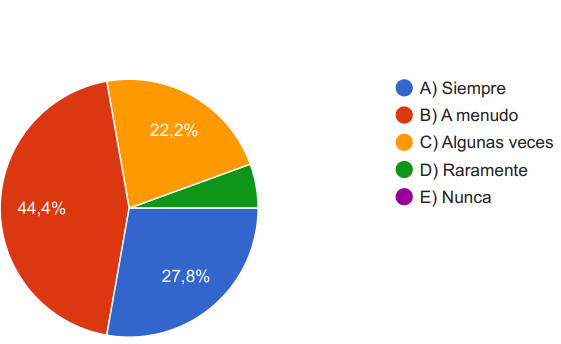
\includegraphics[width=07cm]{Pregunta 1}
	\end{figure}
	\textit{\textbf{Análisis:}Según los resultados obtenidos en esta pregunta, la mayoría de los estudiantes encuestados (44.40\%) informaron reconocer e identificar sus propias emociones a menudo, lo que sugiere una capacidad sólida y frecuente de autorreconocimiento emocional entre los estudiantes. Este hallazgo es respaldado por el 27.08\% de los encuestados que afirmaron hacerlo siempre. Estos porcentajes indican que una proporción significativa de estudiantes es consciente de sus propias emociones en diferentes situaciones académicas y personales.
Por otro lado, Las frecuencias más bajas se observaron en las categorías "Algunas Veces" (22.20\%) y "Raramente" (6.32\%), lo que sugiere que hay una minoría de estudiantes que experimentan dificultades ocasionales en la identificación y reconocimiento de sus emociones. Sin embargo, es alentador notar que ningún encuestado seleccionó la opción "Nunca", lo que indica que todos los estudiantes que participaron tienen al menos algún nivel de capacidad de autorreconocimiento emocional.
}\\

\item ¿Qué tan importante crees que es la comprensión de tus propias emociones para tener éxito en tus estudios y futura carrera profesional como ingeniero de sistemas informáticos?
	\begin{table}[H]
		\renewcommand{\arraystretch}{1.3}
		\centering
		\begin{tabular}{|c|c|c|}
			\hline
			\textbf{Respuestas} & \textbf{Frecuencia} & \textbf{Porcentaje (\%)}\\
			\hline
			Muy Importante & 14 & 77.80 \\
			Importante & 2 & 11.10 \\
			Moderadamente Importante & 2 & 11.10\\
			Poco Importante & 0 & 0.00\\
			Nada Importante & 0 & 0.00\\
			\hline
			\textbf{Totales} &\textbf{18}& \textbf{100.00}\\
			\hline
		\end{tabular}
	\end{table}
	\begin{figure}[h]
		\centering
		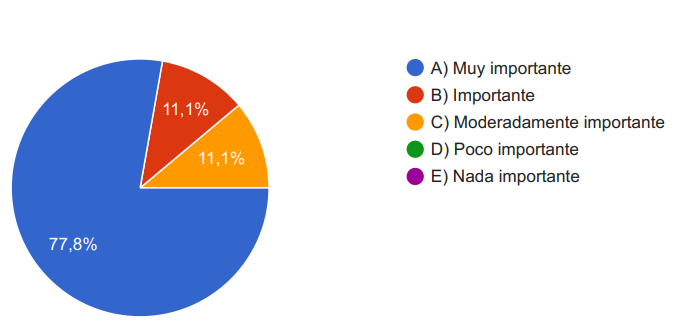
\includegraphics[width=07cm]{Pregunta 2}
	\end{figure}
	\textit{\textbf{Análisis:}Los resultados obtenidos en este ítem, indican que la gran mayoría de los encuestados (77.80\%) consideraron que la comprensión de sus propias emociones es muy importante para tener éxito en sus estudios y futura carrera profesional como ingeniero de sistemas informáticos. Esta alta proporción refleja una valoración positiva y prácticamente unánime de la inteligencia emocional en el ámbito académico y profesional por parte de los estudiantes encuestados.
Además, la importancia otorgada a la comprensión de las emociones indica que los estudiantes reconocen la relevancia de la inteligencia emocional para su éxito en el campo de la ingeniería de sistemas informáticos. Este hallazgo sugiere que los encuestados están conscientes de la influencia de las emociones en su desempeño académico y en su futura carrera profesional, y reconocen la importancia de desarrollar habilidades emocionales para enfrentar eficazmente los desafíos que puedan surgir.
}\\

\item ¿En qué medida sientes que tienes control sobre tus emociones cuando enfrentas desafíos académicos o situaciones estresantes en el contexto universitario?
	\begin{table}[H]
		\renewcommand{\arraystretch}{1.3}
		\centering
		\begin{tabular}{|c|c|c|}
			\hline
			\textbf{Respuestas} & \textbf{Frecuencia} & \textbf{Porcentaje (\%)}\\
			\hline
			Total Control & 10 & 55.60 \\
			Bastante Control & 6 & 33.33 \\
			Algo de Control & 1 & 5.53\\
			Poco Control & 1 & 5.54\\
			Ningún Control & 0 & 0.00\\
			\hline
			\textbf{Totales} &\textbf{18}& \textbf{100.00}\\
			\hline
		\end{tabular}
	\end{table}
	\begin{figure}[h]
		\centering
		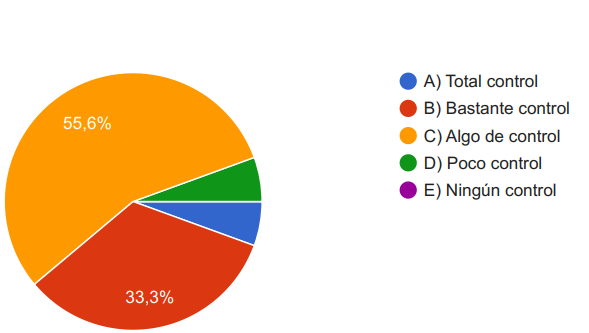
\includegraphics[width=07cm]{Pregunta 3}
	\end{figure}
	\textit{\textbf{Análisis:}Los resultados indica que la mayoría de los encuestados (55.60\%) indicaron tener total control sobre sus emociones cuando enfrentan desafíos académicos o situaciones estresantes en el contexto universitario. Esta alta proporción indica un nivel significativo de autorregulación emocional entre los estudiantes encuestados, lo que podría ser beneficioso para su bienestar y rendimiento académico.
El hecho de que más de la mitad de los encuestados afirmen tener total control sobre sus emociones indica una capacidad sólida para gestionar eficazmente las emociones, incluso en situaciones estresantes. Esto nos sugiere que los estudiantes están equipados con habilidades emocionales que les permiten mantener la calma y tomar decisiones racionales en momentos de presión académica.
Además, el 33.33\% de los encuestados reportaron tener bastante control sobre sus emociones, lo que respalda aún más la idea de que los estudiantes tienen un nivel significativo de autorregulación emocional en el contexto universitario.
}\\

\item¿Consideras que la inteligencia emocional es fundamental para el desarrollo de habilidades profesionales en el campo de la ingeniería de sistemas informáticos?
	\begin{table}[H]
		\renewcommand{\arraystretch}{1.3}
		\centering
		\begin{tabular}{|c|c|c|}
			\hline
			\textbf{Respuestas} & \textbf{Frecuencia} & \textbf{Porcentaje (\%)}\\
			\hline
			Si, es esencial & 13 & 72.20 \\
			Si, es importante & 5 & 27.80 \\
			No estoy seguro/a & 0 & 0.00\\
			No, es poco relevante & 0 & 0.00\\
			No, no es relevante en lo absoluto. & 0 & 0.00\\
			\hline
			\textbf{Totales} &\textbf{18}& \textbf{100.00}\\
			\hline
		\end{tabular}
	\end{table}
	\begin{figure}[h]
		\centering
		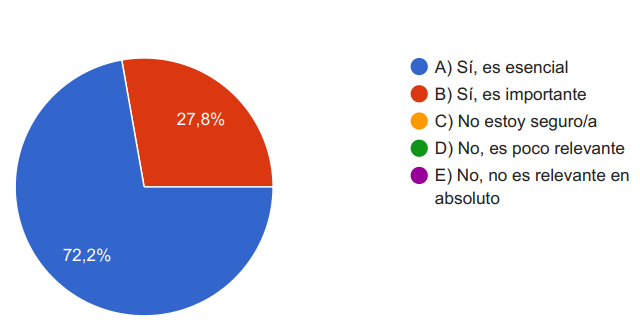
\includegraphics[width=07cm]{Pregunta 4}
	\end{figure}
	\textit{\textbf{Análisis:}Según los resultados obtenidos, la mayoría de los encuestados (72.20\%) consideraron que la inteligencia emocional es esencial para el desarrollo de habilidades profesionales en el campo de la ingeniería de sistemas informáticos. Además, un 27.80\% adicional afirmó que la inteligencia emocional es importante. Estos resultados reflejan una alta valoración de la inteligencia emocional en relación con el desarrollo de habilidades profesionales entre los estudiantes encuestados.
La percepción de que la inteligencia emocional es esencial o importante para el desarrollo de habilidades profesionales sugiere que los estudiantes reconocen la importancia de las habilidades emocionales en el ámbito laboral de la ingeniería de sistemas informáticos. Esto puede interpretarse como una indicación de que los estudiantes encuestados reconocen que las habilidades emocionales, como la capacidad de manejar el estrés, la comunicación efectiva y la resolución de conflictos, son críticas para tener éxito en su futura carrera profesional.
Estos hallazgos insinúan que existe una comprensión generalizada entre los estudiantes encuestados sobre el papel fundamental que desempeña la inteligencia emocional en el desarrollo de habilidades profesionales en el campo de la ingeniería de sistemas informáticos.
}\\

\item¿Crees que la inteligencia emocional puede contribuir al éxito académico?
	\begin{table}[H]
		\renewcommand{\arraystretch}{1.3}
		\centering
		\begin{tabular}{|c|c|c|}
			\hline
			\textbf{Respuestas} & \textbf{Frecuencia} & \textbf{Porcentaje (\%)}\\
			\hline
			Si, definitivamente & 15 & 83.30 \\
			Si, en cierta medida & 3 & 16.70 \\
			No estoy seguro/a & 0 & 0.00\\
			No, no creo que tenga influencia & 0 & 0.00\\
			No, creo que es irrelevante para el éxito académico. & 0 & 0.00\\
			\hline
			\textbf{Totales} &\textbf{18}& \textbf{100.00}\\
			\hline
		\end{tabular}
	\end{table}
	\begin{figure}[h]
		\centering
		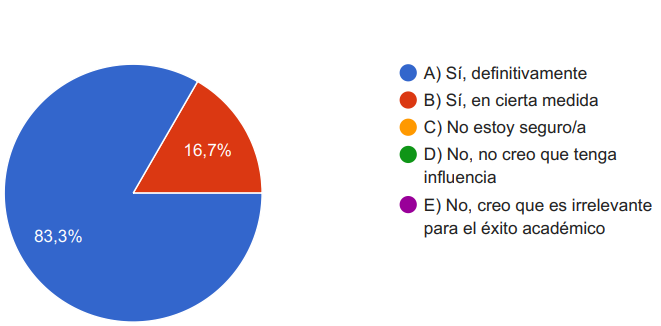
\includegraphics[width=07cm]{Pregunta 5}
	\end{figure}
	\textit{\textbf{Análisis:}Los datos recopilados indican que la gran mayoría de los estudiantes encuestados (83.30\%) creyeron que la inteligencia emocional definitivamente puede contribuir al éxito académico. Además, un 16.70\% adicional indicó que en cierta medida puede tener influencia. Estos resultados reflejan una percepción positiva y generalizada de la inteligencia emocional como un factor importante para el éxito académico entre los estudiantes encuestados.
La alta proporción de estudiantes que creen que la inteligencia emocional definitivamente puede contribuir al éxito académico indica que existe una comprensión sólida y generalizada de la importancia de las habilidades emocionales en el contexto educativo. Esto puede interpretarse como una indicación de que los encuestados reconocen que las habilidades emocionales, como la gestión del estrés, la automotivación y las habilidades de comunicación, son fundamentales para alcanzar el éxito académico.
Además, el hecho de que un porcentaje adicional de encuestados reconozca que la inteligencia emocional puede tener influencia en el éxito académico, aunque no lo vean como definitivo, sugiere que algunos estudiantes pueden estar menos seguros o tener una percepción más matizada de la relación entre la inteligencia emocional y el éxito académico.
}\\

\item ¿Has recibido formación o capacitación específica en inteligencia emocional durante tus estudios de ingeniería de sistemas informáticos?
	\begin{table}[H]
		\renewcommand{\arraystretch}{1.3}
		\centering
		\begin{tabular}{|c|c|c|}
			\hline
			\textbf{Respuestas} & \textbf{Frecuencia} & \textbf{Porcentaje (\%)}\\
			\hline
			Si, de manera regular & 1 & 5.55 \\
			Si, ocasionalmente & 6 & 33.33 \\
			No, pero me gustaría & 10 & 55.60\\
			No, y no creo que sea necesario & 1 & 5.55\\
			No, y no estoy interesado/a en ello & 0 & 0.00\\
			\hline
			\textbf{Totales} &\textbf{18}& \textbf{100.00}\\
			\hline
		\end{tabular}
	\end{table}
	\begin{figure}[h]
		\centering
		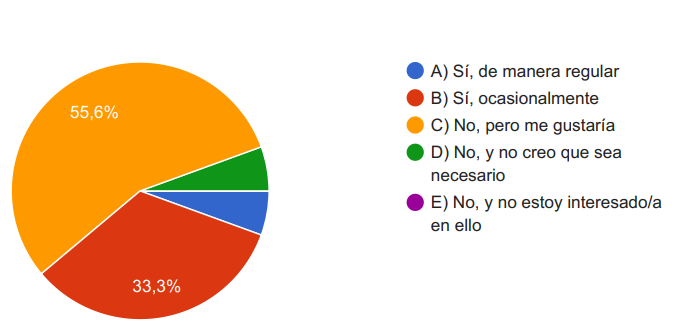
\includegraphics[width=07cm]{Pregunta 6}
	\end{figure}
	\textit{\textbf{Análisis:}Según lo revelado por los estudiantes encuestados, la mayoría (55.60\%) indicaron que no han recibido formación o capacitación específica en inteligencia emocional durante sus estudios de ingeniería de sistemas informáticos. Este hallazgo sugiere que, en general, la inclusión de la inteligencia emocional en el plan de estudios de ingeniería de sistemas informáticos puede ser limitada o insuficiente.
Sin embargo, es alentador notar que un pequeño porcentaje (5.55\%) informó haber recibido formación de manera regular, y un 33.30\% ocasionalmente. Estos resultados indican que algunos estudiantes han tenido acceso a alguna forma de formación en inteligencia emocional durante sus estudios. Esto plantea que existe cierto interés y demanda por parte de los estudiantes en recibir este tipo de capacitación, lo que podría reflejar una comprensión de la importancia de las habilidades emocionales en su desarrollo personal y profesional.
El hecho de que la mayoría de los estudiantes encuestados no hayan recibido formación específica en inteligencia emocional durante sus estudios presenta una oportunidad para integrar más esta formación en el plan de estudios de ingeniería de sistemas informáticos. Al hacerlo, la Escuela de Sistemas podría satisfacer la demanda percibida de los estudiantes y ayudarles a desarrollar habilidades emocionales que sean relevantes y beneficiosas para su éxito académico y profesional en el campo de la ingeniería de sistemas informáticos.
}\\

\item¿Cómo crees que la inteligencia emocional podría impactar tu desempeño en el campo laboral relacionado con la ingeniería de sistemas informáticos?
	\begin{table}[H]
		\renewcommand{\arraystretch}{1.3}
		\centering
		\begin{tabular}{c c c}
			\hline
			\textbf{Respuestas} & \textbf{Frecuencia} & \textbf{Porcentaje (\%)}\\
			\hline
			Mejoraría mi capacidad \\de trabajo en equipo & 3 & 16.70 \\
			\\Me ayudaría a gestionar \\mejor el estrés laboral & 10 & 55.60 \\
			\\Facilitaría la resolución\\ de conflictos en el trabajo & 5 & 27.80\\
			\\No estoy seguro/a & 0 & 0.00\\
			\\No creo que tenga impacto\\ en mi desempeño laboral & 0 & 0.00\\
			\hline
			\textbf{Totales} &\textbf{18}& \textbf{100.00}\\
			\hline
		\end{tabular}
	\end{table}
	\begin{figure}[h]
		\centering
		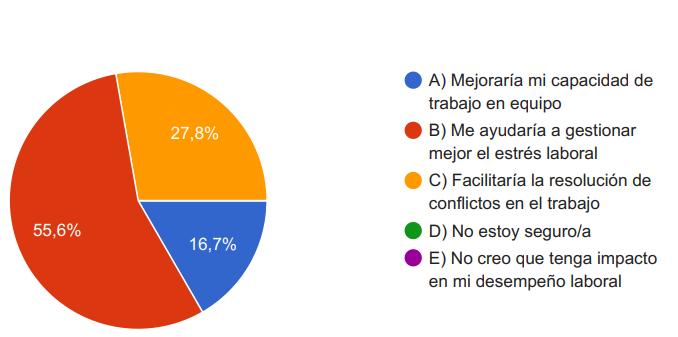
\includegraphics[width=07cm]{Pregunta 7}
	\end{figure}
	\textit{\textbf{Análisis:}los resultados indican que la mayoría de los estudiantes encuestados identificaron que la inteligencia emocional podría impactar positivamente su desempeño en el campo laboral relacionado con la ingeniería de sistemas informáticos. En detalle:
Un 55.60\% de los encuestados indicaron que la inteligencia emocional les ayudaría a gestionar mejor el estrés laboral.
Un 27.80\% señalaron que facilitaría la resolución de conflictos en el trabajo.
Un 16.70\% mencionaron que mejoraría su capacidad de trabajo en equipo.
Estos resultados sugieren que los estudiantes reconocen el valor de la inteligencia emocional en el entorno laboral y esperan que les ayude a enfrentar los desafíos comunes en su futura carrera profesional.
La alta proporción de estudiantes encuestados que identificaron la capacidad de la inteligencia emocional para mejorar la gestión del estrés laboral es especialmente notable, lo que indica una comprensión generalizada de la importancia de esta habilidad en un campo laboral que puede ser altamente exigente y estresante, como la ingeniería de sistemas informáticos.
Además, el reconocimiento de que la inteligencia emocional puede facilitar la resolución de conflictos en el trabajo y mejorar la capacidad de trabajo en equipo sugiere una comprensión de cómo estas habilidades emocionales pueden contribuir al éxito en entornos laborales colaborativos y orientados a proyectos, comunes en el campo de la ingeniería de sistemas informáticos.
}\\

\item¿Cómo crees que la inteligencia emocional influye en tu capacidad para resolver problemas de manera efectiva y colaborativa en los equipos de trabajo durante tus estudios de ingeniería de sistemas informáticos?
	\begin{table}[H]
		\renewcommand{\arraystretch}{1.3}
		\centering
		\begin{tabular}{c c c}
			\hline
			\textbf{Respuestas} & \textbf{Frecuencia} & \textbf{Porcentaje (\%)}\\
			\hline
			Mejora significativamente \\mi capacidad de resolución \\de problemas en equipo. & 16 & 88.90 \\
			\\Tiene un impacto positivo, \\pero no es determinante & 2 & 11.10 \\
			\\No estoy seguro/a & 0 & 0.00\\
			\\No creo que tenga influencia \\en mi capacidad para \\resolver problemas en equipo. & 0 & 0.00\\
			\\Creo que puede dificultar la \\resolución de problemas \\en equipo. & 0 & 0.00\\
			\hline
			\textbf{Totales} &\textbf{18}& \textbf{100.00}\\
			\hline
		\end{tabular}
	\end{table}
	\begin{figure}[h]
		\centering
		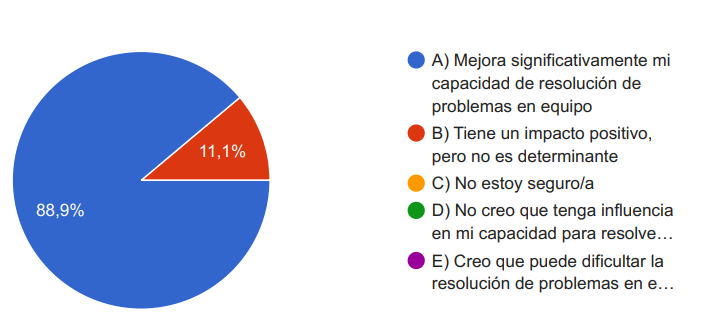
\includegraphics[width=07cm]{Pregunta 8}
	\end{figure}
	\textit{\textbf{Análisis:}Según los resultados obtenidos, la mayoría abrumadora de los estudiantes encuestados (88.90\%) consideró que la inteligencia emocional mejora significativamente su capacidad para resolver problemas de manera efectiva y colaborativa en los equipos de trabajo durante sus estudios.
Solo un pequeño porcentaje (11.10\%) indicó que la inteligencia emocional tiene un impacto positivo, pero no es determinante.
Estos resultados reflejan una clara percepción entre los estudiantes encuestados de que la inteligencia emocional juega un papel crucial en la resolución de problemas en entornos de trabajo en equipo, esto indica una comprensión generalizada de la importancia de las habilidades emocionales en el ámbito estudiantil.
La alta proporción de encuestados que atribuyen a la inteligencia emocional una mejora significativa en la resolución de problemas en equipo sugiere que los estudiantes valoran la capacidad de comprensión emocional y comunicación efectiva cuando se trata de colaboración, aspectos fundamentales en el desarrollo de soluciones efectivas y la productividad en equipos de trabajo.
}\\

\item¿Cómo consideras que la inteligencia emocional puede influir en la eficacia de tu contribución a un equipo de desarrollo de software o proyecto relacionado con la ingeniería de sistemas informáticos?
	\begin{table}[H]
		\renewcommand{\arraystretch}{1.3}
		\centering
		\begin{tabular}{c c c}
			\hline
			\textbf{Respuestas} & \textbf{Frecuencia} & \textbf{Porcentaje (\%)}\\
			\hline
			Mejora mi capacidad \\para comunicarme\\ y colaborar con otros miembros\\ del equipo & 10 & 55.60 \\
			\\Me ayuda a manejar \\mejor las situaciones\\ de conflicto dentro \\del equipo & 8 & 44.40 \\
			\\No estoy seguro/a. & 0 & 0.00\\
			\\No creo que tenga \\impacto en \\mi contribución al equipo & 0 & 0.00\\
			\\Creo que podría ser\\ una distracción y afectar\\ negativamente mi contribución \\al equipo & 0 & 0.00\\
			\hline
			\textbf{Totales} &\textbf{18}& \textbf{100.00}\\
			\hline
		\end{tabular}
	\end{table}
	\begin{figure}[h]
		\centering
		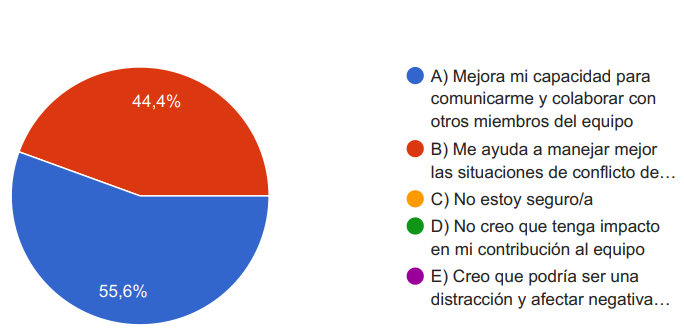
\includegraphics[width=07cm]{Pregunta 9}
	\end{figure}
	\textit{\textbf{Análisis:}Los datos recolectados indican que la mayoría de los encuestados (55.60\%) indicaron que la inteligencia emocional mejora significativamente su capacidad para comunicarse y colaborar con otros miembros del equipo en proyectos relacionados con la ingeniería de sistemas informáticos.
Un porcentaje significativo (44.40\%) indicó que la inteligencia emocional les ayuda a manejar mejor las situaciones de conflicto dentro del equipo.
Estos resultados manifiestan que los estudiantes reconocen la influencia positiva de la inteligencia emocional en la eficacia de su contribución a los equipos de desarrollo de software o proyectos relacionados con la ingeniería de sistemas informáticos, particularmente en términos de mejora en la comunicación, colaboración y manejo de conflictos.
La alta proporción de encuestados que identificaron que la inteligencia emocional mejora la capacidad de comunicación y colaboración en equipo sugiere que los estudiantes valoran la capacidad de comprensión emocional y la habilidad para trabajar eficazmente en conjunto en el contexto de proyectos complejos que se realizan en ciertas materias de la carrea de ingeniería de sistemas informáticos.
Además, el reconocimiento de que la inteligencia emocional ayuda a manejar mejor las situaciones de conflicto dentro del equipo resalta la importancia de estas habilidades emocionales en la resolución de disputas y mantenimiento de un ambiente de trabajo armonioso y productivo, aspectos cruciales en el éxito de los proyectos de ingeniería de sistemas informáticos.
}\\

\item¿Qué aspectos de la inteligencia emocional consideras más importantes para tener éxito en proyectos de ingeniería de sistemas informáticos que requieren trabajo en equipo?
	\begin{table}[H]
		\renewcommand{\arraystretch}{1.3}
		\centering
		\begin{tabular}{c c c}
			\hline
			\textbf{Respuestas} & \textbf{Frecuencia} & \textbf{Porcentaje (\%)}\\
			\hline
			Autoconocimiento y \\autorregulación emocional  & 6 & 33.30 \\
			\\Empatía y habilidades \\sociales  & 1 & 5.55 \\
			\\Ambas son igualmente \\importantes  & 10 & 55.60\\
			\\No estoy seguro/a  & 1 & 5.55\\
			\\No creo que la inteligencia \\emocional sea relevante \\para el éxito en \\proyectos de equipo & 0 & 0.00\\
			\hline
			\textbf{Totales} &\textbf{18}& \textbf{100.00}\\
			\hline
		\end{tabular}
	\end{table}
	\begin{figure}[h]
		\centering
		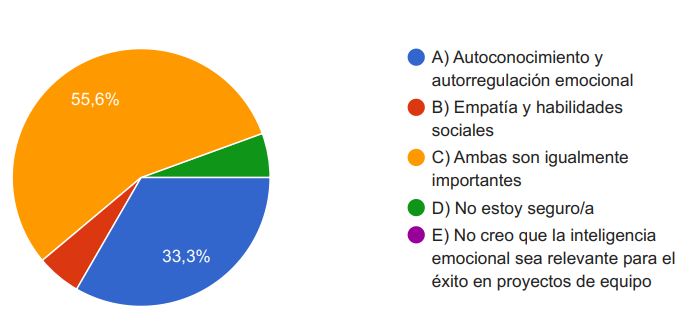
\includegraphics[width=07cm]{Pregunta10}
	\end{figure}
	\textit{\textbf{Análisis:}Los resultados indican que una mayoría abrumadora de los estudiantes encuestados (55.60\%) consideró que tanto el autoconocimiento y la autorregulación emocional como la empatía y las habilidades sociales son igualmente importantes para tener éxito en proyectos de ingeniería de sistemas informáticos que requieren trabajo en equipo.
Un 33.30\% indicó que ambas son igualmente importantes, mientras que un 5.55\% consideró que el autoconocimiento y la autorregulación emocional son más relevantes y un 5.55\% no estaba seguro/a.
Estos resultados subrayan la percepción generalizada entre los estudiantes de la importancia de una amplia gama de habilidades emocionales, como el autoconocimiento, la autorregulación, la empatía y las habilidades de comunicación, para tener éxito en proyectos de equipo en el campo de la ingeniería de sistemas informáticos.
El reconocimiento de la igual importancia de ambas categorías de habilidades emocionales sugiere una comprensión profunda de cómo estas pueden interactuar y complementarse entre sí para optimizar la dinámica y eficacia de los equipos de trabajo en proyectos complejos.
}\\

\item¿Cómo percibes tus niveles de estrés en el contexto de tus estudios de ingeniería de sistemas informáticos?
	\begin{table}[H]
		\renewcommand{\arraystretch}{1.3}
		\centering
		\begin{tabular}{|c|c|c|}
			\hline
			\textbf{Respuestas} & \textbf{Frecuencia} & \textbf{Porcentaje (\%)}\\
			\hline
			Muy altos & 5 & 27.80 \\
			Altos & 4 & 22.20 \\
			Moderados & 8 & 44.40\\
			Bajos & 1 & 5.60\\
			Muy bajos & 0 & 0.00\\
			\hline
			\textbf{Totales} &\textbf{18}& \textbf{100.00}\\
			\hline
		\end{tabular}
	\end{table}
	\begin{figure}[h]
		\centering
		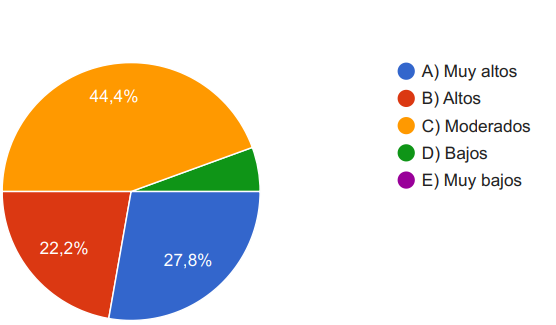
\includegraphics[width=07cm]{Pregunta11}
	\end{figure}
	\textit{\textbf{Análisis:}En los resultados recolectados se observa una distribución variada en cuanto a la percepción de los niveles de estrés entre los estudiantes de ingeniería de sistemas informáticos. Además de estos hallazgos, es importante considerar el papel que la inteligencia emocional puede desempeñar en la gestión y percepción del estrés en este contexto académico.
La correlación entre la inteligencia emocional y la capacidad para manejar el estrés de forma eficaz siempre han ido de la mano, La capacidad de reconocer, comprender y regular las propias emociones, así como la habilidad para manejar las relaciones interpersonales, son componentes clave de la inteligencia emocional que pueden influir en la forma en que los estudiantes enfrentan situaciones estresantes.
En este sentido, los resultados obtenidos pueden interpretarse a la luz de la inteligencia emocional. Por ejemplo, es posible que aquellos estudiantes que reportaron niveles de estrés moderados o altos también puedan beneficiarse de un mayor desarrollo de habilidades emocionales para gestionar de manera más efectiva estas experiencias estresantes. Por otro lado, la ausencia de estudiantes que reportaron niveles de estrés muy bajos puede indicar una oportunidad para integrar más formación en inteligencia emocional en el plan de estudios de la carrera, con el objetivo de proporcionar a los estudiantes herramientas adicionales para gestionar el estrés de manera más efectiva.
}\\

\item¿Crees que la inteligencia emocional puede desempeñar un papel importante en el manejo del estrés durante tus estudios de ingeniería de sistemas informáticos?
	\begin{table}[H]
		\renewcommand{\arraystretch}{1.3}
		\centering
		\begin{tabular}{c c c}
			\hline
			\textbf{Respuestas} & \textbf{Frecuencia} & \textbf{Porcentaje (\%)}\\
			\hline
			Si, definitivamente & 13 & 72.20 \\
			Si, en cierta manera & 4 & 22.20 \\
			No estoy seguro/a & 1 & 5.60\\
			No, no creo que tenga influencia & 0 & 0.00\\
			\\No, creo que es\\ irrelevante para el\\ manejo de estrés. & 0 & 0.00\\
			\hline
			\textbf{Totales} &\textbf{18}& \textbf{100.00}\\
			\hline
		\end{tabular}
	\end{table}
	\begin{figure}[h]
		\centering
		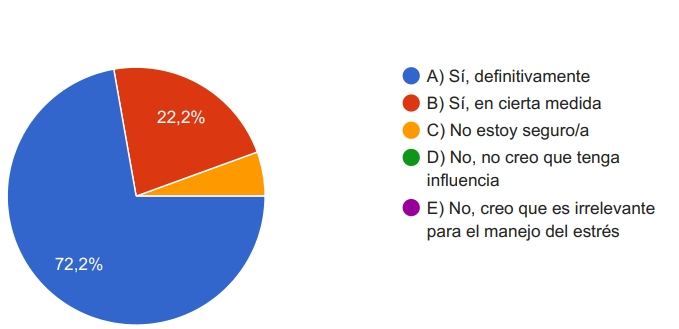
\includegraphics[width=07cm]{Pregunta12}
	\end{figure}
	\textit{\textbf{Análisis:}Los resultados de la encuesta revelan una percepción mayoritariamente positiva entre los estudiantes de ingeniería de sistemas informáticos sobre el papel de la inteligencia emocional en el manejo del estrés durante sus estudios:
Un 72.20\% de los encuestados afirmaron que la inteligencia emocional definitivamente puede desempeñar un papel importante en el manejo del estrés.
Un 22.20\% indicaron que en cierta manera la inteligencia emocional podría influir en el manejo del estrés.
Solo un 5.60\% manifestó estar indeciso sobre la influencia de la inteligencia emocional en el manejo del estrés.
Estos resultados reflejan una clara tendencia hacia la percepción positiva de la inteligencia emocional como una herramienta relevante para afrontar el estrés en el contexto de los estudios de ingeniería de sistemas informáticos. La mayoría de los estudiantes reconocen la importancia de las habilidades emocionales para manejar eficazmente las presiones y demandas académicas asociadas con esta disciplina.
}\\
	\item ¿Cómo evalúas la comunicación dentro de los equipos de proyectos de TI en los que has participado (ya sea en tu trabajo o proyectos de ciclo)?
	\begin{table}[H]
		\renewcommand{\arraystretch}{1.3}
		\centering
		\begin{tabular}{|c|c|c|}
			\hline
			\textbf{Respuestas} & \textbf{Frecuencia} & \textbf{Porcentaje (\%)}\\
			\hline
			Excelente & 4 & 22.22 \\
			Buena & 11 & 61.11 \\
			Regular & 2 & 11.11\\
			Deficiente & 1 & 5.56\\
			\hline
			\textbf{Totales} &\textbf{18}& \textbf{100.00}\\
			\hline
		\end{tabular}
	\end{table}
	\begin{figure}[h]
		\centering
		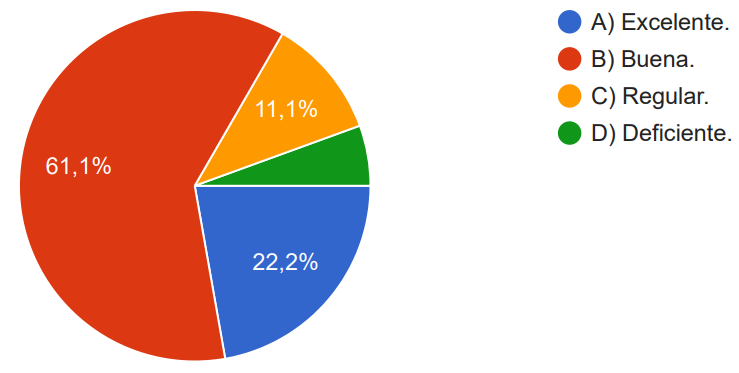
\includegraphics[width=07cm]{Pregunta13}
	\end{figure}
	\textit{\textbf{Análisis:} La mayoría de los encuestados (61.11\%) califican la comunicación como buena, mientras que un 22.22\% la considera excelente. Esto indica una percepción general positiva de la comunicación dentro de los equipos. Aunque las respuestas son mayormente positivas, un 16.67\% de los participantes cree que la comunicación es regular o deficiente, lo que señala oportunidades para mejorar.}\\
	
	\item ¿Tu líder brinda la atención adecuada cuando te diriges a él o ella para tratar algún tema?
	\begin{enumerate}
		\item Sí, siempre.
		\item A veces.
		\item No, nunca.
	\end{enumerate}
	\begin{table}[H]
		\renewcommand{\arraystretch}{1.3}
		\centering
		\begin{tabular}{|c|c|c|}
			\hline
			\textbf{Respuestas} & \textbf{Frecuencia} & \textbf{Porcentaje (\%)}\\
			\hline
			Sí, siempre & 11 & 61.11\\
			A veces & 6 & 33.33\\
			No, nunca & 1 &	5.56\\	
			\hline
			\textbf{Totales} &\textbf{18}& \textbf{100.00}\\
			\hline
		\end{tabular}
	\end{table}
	\begin{figure}[h]
		\centering
		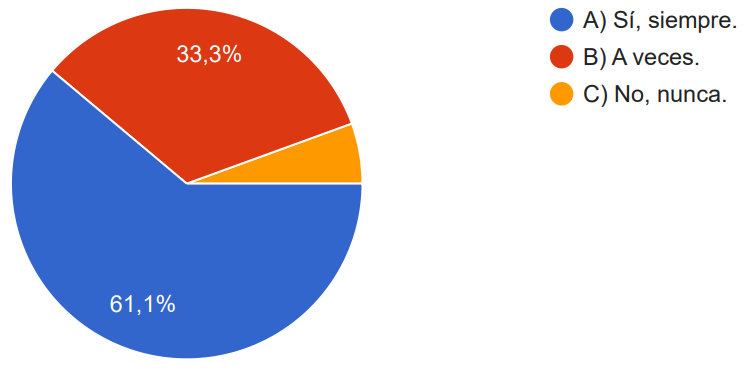
\includegraphics[width=06cm]{Pregunta14}
	\end{figure}
	\textit{\textbf{Análisis:} La mayoría (61.11\%) siente que siempre recibe la atención adecuada de su líder, mientras que un 33.33\% la recibe a veces, indicando que la consistencia en la atención por parte de los líderes podría ser un área a desarrollar. Solo un 5.56\% reporta nunca recibir la atención adecuada, lo cual podría requerir atención individualizada para entender y abordar estas situaciones específicas.}\\
	
	\item ¿Crees que los comentarios o sugerencias que aportas son tomados en cuenta?
	\begin{enumerate}
		\item Sí, siempre.
		\item En ocasiones.
		\item No, nunca.
	\end{enumerate}
	\begin{table}[H]
		\renewcommand{\arraystretch}{1.3}
		\centering
		\begin{tabular}{|c|c|c|}
			\hline
			\textbf{Respuestas} & \textbf{Frecuencia} & \textbf{Porcentaje (\%)}\\
			\hline
			Sí, siempre & 9 & 50.00\\
			En ocasiones & 9 & 50.00\\
			No, nunca & 0 & 0.00\\
			\hline
			\textbf{Totales} &\textbf{18}& \textbf{100.00}\\
			\hline
		\end{tabular}
	\end{table}
	\begin{figure}[h]
		\centering
		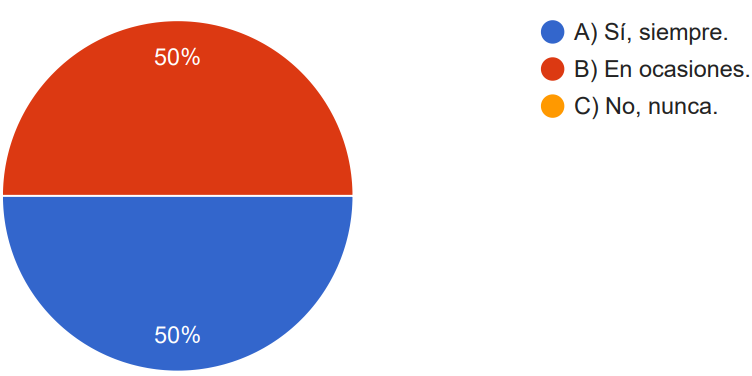
\includegraphics[width=06cm]{Pregunta15}
	\end{figure}
	\textit{\textbf{Análisis:} Un 50\% afirma que sus aportes siempre son considerados, lo que indica una apertura positiva a la retroalimentación. El otro 50\% siente que sus comentarios son tomados en cuenta en ocasiones, lo que sugiere que hay momentos en los que la comunicación podría ser más efectiva o que algunos aportes no se están valorando adecuadamente. Es notable que no hay respuestas que indiquen una falta total de consideración (0\% para “No, nunca”), lo cual es un aspecto positivo}\\

	\item ¿Sientes que cuentas con la confianza y libertad de tus superiores para discutir algún problema de trabajo?
	\begin{enumerate}
		\item Totalmente.
		\item En cierta medida.
		\item No en absoluto.
	\end{enumerate}
	\begin{table}[H]
		\renewcommand{\arraystretch}{1.3}
		\centering
		\begin{tabular}{|c|c|c|}
			\hline
			\textbf{Respuestas} & \textbf{Frecuencia} & \textbf{Porcentaje (\%)}\\
			\hline
			Totalmente & 7 & 38.89\\
			En cierta medida & 11 & 61.11\\
			No en absoluto & 0 & 0.00\\
			\hline
			\textbf{Totales} &\textbf{18}& \textbf{100.00}\\
			\hline
		\end{tabular}
	\end{table}
	\begin{figure}[h]
		\centering
		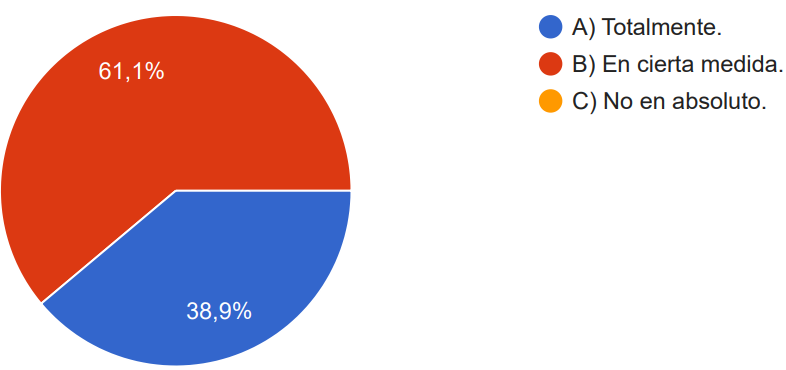
\includegraphics[width=06cm]{Pregunta16}
	\end{figure}
	\textit{\textbf{Análisis:} Un 38.89\% de los encuestados siente que tiene totalmente la confianza y libertad de sus superiores para discutir problemas laborales. La mayoría, un 61.11\%, indica que siente esta confianza en cierta medida, lo que podría sugerir que hay espacio para mejorar la comunicación abierta y la confianza entre miembros del equipo y el líder.}\\
	
	\item ¿Qué cualidades crees que debe tener un buen líder en proyectos de TI?
	\begin{enumerate}
		\item Empatía.
		\item Habilidades de resolución de problemas.
		\item Comunicación efectiva.
		\item Capacidad para motivar al equipo.
	\end{enumerate}
	\begin{table}[H]
		\renewcommand{\arraystretch}{1.3}
		\centering
		\begin{tabular}{|c|c|c|}
			\hline
			\textbf{Respuestas} & \textbf{Frecuencia} & \textbf{Porcentaje (\%)}\\
			\hline
			Empatía & 1 & 5.56\\
			Habilidades de resolución de problemas & 8 & 44.44\\
			Comunicación efectiva & 6 & 33.33\\
			Capacidad para motivar al equipo & 3 & 16.67\\
			\hline
			\textbf{Totales} &\textbf{18}& \textbf{100.00}\\
			\hline
		\end{tabular}
	\end{table}
	\begin{figure}[h]
		\centering
		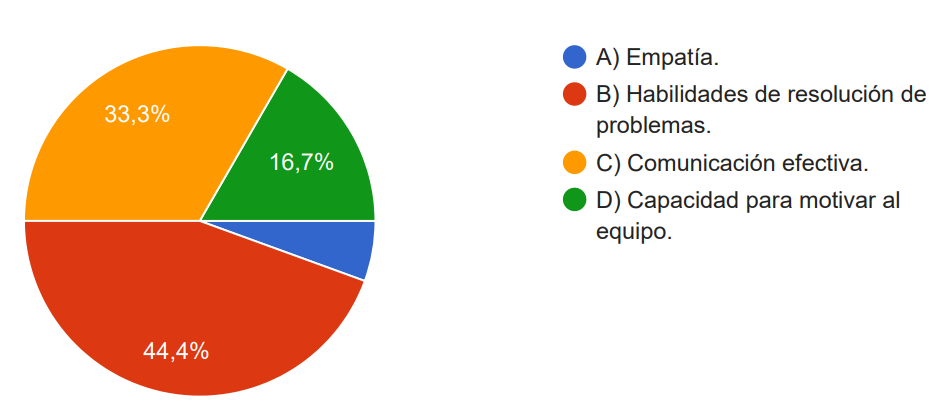
\includegraphics[width=07cm]{Pregunta17}
	\end{figure}
	\textit{\textbf{Análisis:} Un 44.44\% considera la habilidad de resolución de problemas como la cualidad más valorada, lo que indica que la capacidad para enfrentar y solucionar desafíos es esencial para un líder en TI. Por otra parte, un 33.33\% indica que la comunicación clara y efectiva es crucial para la coordinación y el éxito del equipo. Luego, un 22.23\% responde que un líder debe ser capaz de motivar a su equipo para alcanzar sus objetivos comunes y entender las emociones de los demás para crear un ambiente de trabajo positivo y colaborativo.}\\
		
	\item ¿Has tenido un líder que elogia tus habilidades y expresa lo bueno de tu trabajo?
	\begin{enumerate}
		\item Si
		\item No
	\end{enumerate}
	\begin{table}[H]
		\renewcommand{\arraystretch}{1.3}
		\centering
		\begin{tabular}{|c|c|c|}
			\hline
			\textbf{Respuestas} & \textbf{Frecuencia} & \textbf{Porcentaje (\%)}\\
			\hline
			Sí & 16 & 88.89\\
			No & 2 & 11.11\\
			\hline
			\textbf{Totales} &\textbf{18}& \textbf{100.00}\\
			\hline
		\end{tabular}
	\end{table}
	\begin{figure}[h]
		\centering
		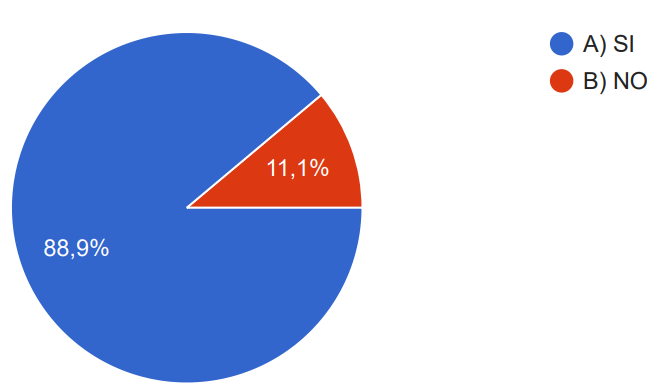
\includegraphics[width=06cm]{Pregunta18}
	\end{figure}
	\textit{\textbf{Análisis:} Se observa que la gran mayoría de los encuestados (88.89\%) han tenido líderes que elogian sus habilidades y expresan lo bueno de su trabajo. Esto sugiere que el reconocimiento y la valoración positiva son prácticas comunes en su entorno laboral. Por otro lado, un 11.11\% indica que no han recibido este tipo de retroalimentación, lo cual podría ser un área de oportunidad para mejorar la moral y motivación del equipo.}\\
	
	\item ¿En alguna ocasión te han llamado la atención de forma indirecta resultando ser útil sin causarte resentimiento?
	\begin{enumerate}
		\item Si
		\item No
	\end{enumerate}
	\begin{table}[H]
		\renewcommand{\arraystretch}{1.3}
		\centering
		\begin{tabular}{|c|c|c|}
			\hline
			\textbf{Respuestas} & \textbf{Frecuencia} & \textbf{Porcentaje (\%)}\\
			\hline
			Sí & 10 & 55.56\\
			No & 8 & 44.44\\
			\hline
			\textbf{Totales} &\textbf{18}& \textbf{100.00}\\
			\hline
		\end{tabular}
	\end{table}
	\begin{figure}[h]
		\centering
		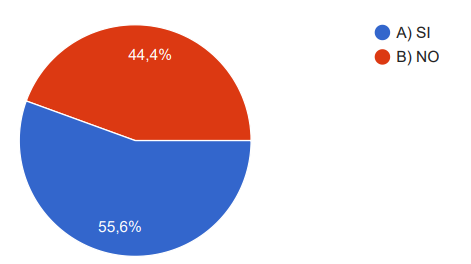
\includegraphics[width=06cm]{Pregunta19}
	\end{figure}
	\textit{\textbf{Análisis:} Más de la mitad de los participantes (55.56\%) han experimentado una retroalimentación indirecta que resultó ser útil sin causar resentimiento. Esto sugiere que la retroalimentación constructiva, cuando se entrega de manera adecuada, puede ser efectiva y bien recibida. Por otro lado, un 44.44\% no ha tenido la misma experiencia, lo que podría indicar la necesidad de mejorar las técnicas de comunicación para asegurar que los mensajes críticos sean entregados de una manera que sea percibida como útil y no ofensiva.}\\
	
	\item ¿Cómo describirías la cultura organizacional en tu facultad o lugar de trabajo específicamente para los ingenieros de sistemas informáticos?
	\begin{enumerate}
		\item Colaborativa.
		\item Jerárquica.
		\item Innovadora.
		\item Tradicional.
	\end{enumerate}
	\begin{table}[H]
		\renewcommand{\arraystretch}{1.3}
		\centering
		\begin{tabular}{|c|c|c|}
			\hline
			\textbf{Respuestas} & \textbf{Frecuencia} & \textbf{Porcentaje (\%)}\\
			\hline
			Colaborativa & 6 & 33.33\\
			Jerárquica & 7 & 38.89\\
			Innovadora & 1 & 5.56\\
			Tradicional & 4 & 22.22\\
			\hline
			\textbf{Totales} &\textbf{18}& \textbf{100.00}\\
			\hline
		\end{tabular}
	\end{table}
	\begin{figure}[h]
		\centering
		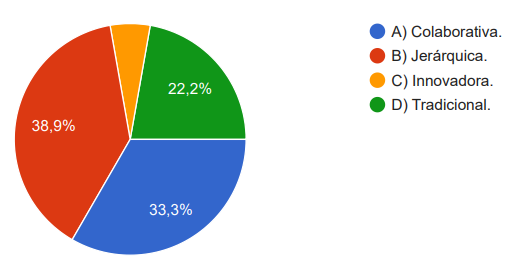
\includegraphics[width=07cm]{Pregunta20}
	\end{figure}
	\textit{\textbf{Análisis:} Según los resultados de la encuesta, es predominantemente jerárquica, con un 38.89\% que la describen así, esto sugiere una estructura donde las decisiones son tomadas por los niveles superiores. Sin embargo, un 33.33\% la considera colaborativa, indicando que la cooperación entre compañeros es también un aspecto significativo. Un 22.22\% la ve como tradicional, lo que podría implicar la presencia de prácticas y procesos bien establecidos. Por último, solo un 5.56\% la percibe como innovadora, lo que señala una oportunidad para fomentar un entorno más creativo y abierto a nuevas ideas.}\\
	
	\item ¿Qué aspectos de la cultura organizacional contribuyen al bienestar y la satisfacción de los empleados en el área de TI?
	\begin{enumerate}
		\item Flexibilidad horaria.
		\item Reconocimiento.
		\item Oportunidades de desarrollo.
		\item Ambiente inclusivo.
	\end{enumerate}
	\begin{table}[H]
	\renewcommand{\arraystretch}{1.3}
	\centering
	\begin{tabular}{|c|c|c|}
		\hline
		\textbf{Respuestas} & \textbf{Frecuencia} & \textbf{Porcentaje (\%)}\\
		\hline
		Flexibilidad horaria & 5 & 27.78\\
		Reconocimiento & 5 & 27.78\\
		Oportunidades de desarrollo & 7 & 38.89\\
		Ambiente inclusivo & 1 & 5.56\\
		\hline
		\textbf{Totales} &\textbf{18}& \textbf{100.00}\\
		\hline
	\end{tabular}
	\end{table}
	\begin{figure}[h]
		\centering
		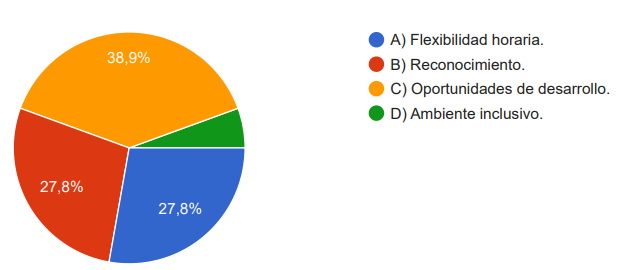
\includegraphics[width=07cm]{Pregunta21}
	\end{figure}
	\textit{\textbf{Análisis:} Los aspectos que más contribuyen al bienestar y satisfacción de los empleados en el área de TI son las oportunidades de desarrollo profesional, valoradas por un 38.89\% de los encuestados, seguidas de la flexibilidad horaria y el reconocimiento, ambos con un 27.78\%. Aunque menos mencionado, con un 5.56\%, un ambiente inclusivo también se considera importante.}\\
	
	\item ¿Qué cambios sugerirías para mejorar el ambiente de trabajo y la colaboración en equipos de desarrollo de software?
	\begin{enumerate}
		\item Mayor apoyo en formación.
		\item Fomentar la diversidad.
		\item Mejorar la comunicación interna.
		\item Reducir la carga de trabajo.
	\end{enumerate}
	\begin{table}[H]
		\renewcommand{\arraystretch}{1.3}
		\centering
		\begin{tabular}{|c|c|c|}
			\hline
			\textbf{Respuestas} & \textbf{Frecuencia} & \textbf{Porcentaje (\%)}\\
			\hline
			Mayor apoyo en formación & 5 & 27.78\\
			Fomentar la diversidad & 1 & 5.56\\
			Mejorar la comunicación interna & 11 & 61.11\\
			Reducir la carga de trabajo & 1 & 5.56\\
			\hline
			\textbf{Totales} &\textbf{18}& \textbf{100.00}\\
			\hline
		\end{tabular}
	\end{table}
	\begin{figure}[h]
		\centering
		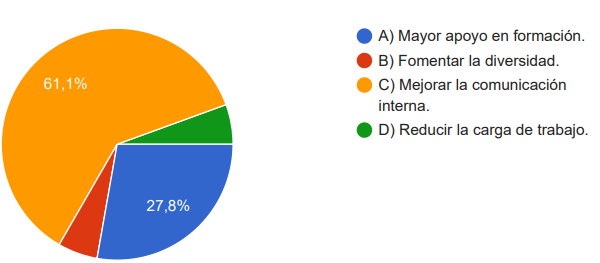
\includegraphics[width=07cm]{Pregunta22}
	\end{figure}
	\textit{\textbf{Análisis:} Los encuestados sugieren principalmente mejorar la comunicación interna (61.11\%), lo que indica que una comunicación clara y efectiva es fundamental. Además, un mayor apoyo en formación (27.78\%) podría ayudar a los empleados a desarrollar habilidades y adaptarse a cambios tecnológicos. Aunque menos mencionados, fomentar la diversidad y reducir la carga de trabajo, ambos con un 5.56\%, también son cambios que podrían contribuir a un mejor clima laboral.}\\
	
\end{enumerate}

\subsection{Procedimiento de recolección de datos}
La recolección de datos se llevará a cabo de manera estructurada y sistemática para garantizar la validez y fiabilidad de los resultados obtenidos. El procedimiento de recolección de datos se realizará en varias etapas:

\begin{enumerate}
	\item \textbf{Etapa 1:} Antes de la implementación, se finalizará y validarán las preguntas de la encuesta diseñadas para abordar los objetivos de investigación. Se garantizará que las preguntas sean claras, comprensibles y relevantes para la temática de estudio.
	\item \textbf{Etapa 2:} La encuesta se administrará de forma voluntaria a los estudiantes de Ingeniería de Sistemas Informáticos en la Universidad De El Salvador, Cede Central. Se utilizará la plataforma en línea Google forms para llegar a la población objetivo.
	\item \textbf{Etapa 3:} Durante el periodo de recolección de datos, se registrarán las respuestas de los participantes de manera precisa y completa. Se garantizará la confidencialidad y privacidad de la información recopilada en todo momento.
	\item \textbf{Etapa 4:} Una vez completada la recolección de datos, se procederá a realizar un análisis estadístico de los datos recopilados. Se utilizarán técnicas de análisis descriptivo e inferencial para examinar las relaciones entre variables y responder a los objetivos de investigación planteados. 
\end{enumerate}

\section{Conclusion}
\begin{center}
	\textbf{Conciencia Emocional}
\end{center}
La mayoría de los estudiantes de Ingeniería de Sistemas Informáticos en la Universidad De El Salvador poseen una sólida capacidad para identificar y reconocer sus propias emociones en diversas situaciones académicas y personales. Esto indica un nivel saludable de conciencia emocional entre los estudiantes encuestados. Esta capacidad de autorreconocimiento emocional es una base importante para el desarrollo de habilidades interpersonales y la gestión efectiva del estrés durante los estudios y futura carrera profesional.
\begin{center}
	\textbf{Relevancia de la inteligencia Emocional}
\end{center}
En base a los resultados obtenidos en la encuesta, concluimos que los estudiantes de Ingeniería de Sistemas Informáticos de la Universidad De El Salvador reconocen la importancia de la inteligencia emocional en diversos aspectos de su formación y desarrollo profesional, en primer lugar, se evidencia que los estudiantes tienen una sólida capacidad para identificar y reconocer sus propias emociones en situaciones tanto académicas como personales, esto indica un nivel significativo de conciencia emocional entre la comunidad estudiantil, en segundo lugar, la gran mayoría de los estudiantes considera que la inteligencia emocional es esencial para el desarrollo de habilidades profesionales y el éxito académico en su carrera. Esta percepción resalta la necesidad de integrar la formación de inteligencia emocional en el pensum académico para satisfacer las expectativas y demandas de los estudiantes, ya que indicaron que no han recibido este tipo de formación durante el desarrollo de la carrera.
\begin{center}
	\textbf{Influencia en la resolución de problemas}
\end{center}
Los estudiantes reconocen la influencia significativa de la inteligencia emocional en su capacidad para resolver problemas de manera efectiva y colaborativa en equipos de trabajo, especialmente en proyectos relacionados con la informática. La mayoría de los encuestados consideraron que la inteligencia emocional mejora significativamente su capacidad para trabajar en equipo y resolver conflictos, lo que destaca la importancia de estas habilidades emocionales en entornos laborales colaborativos y orientados a proyectos.
\begin{center}
	\textbf{Manejo de estrés y bienestar emocional}
\end{center}
Entorno a este punto concluimos que los estudiantes poseen una distribución variada en cuanto a la percepción de los niveles de estrés. Ya que algunos experimentan niveles de estrés moderados o altos, esto en entornos académicos y las exigencias de la carrera que generan un nivel considerable de estrés. Sin embargo, los estudiantes reconocen la importancia de la inteligencia emocional en el manejo del estrés, ya que identificaron la necesidad de desarrollar habilidades emocionales para promover el bienestar emocional durante sus estudios universitarios.

\begin{center}
	\textbf{Eficacia de la comunicación}
\end{center}
Sea demostrado que la comunicación es fundamental en área de informática y que los estudiantes de estas carrera deben ser formados con mucho cuidado en la interacción de personas. El éxito del proyecto es influenciado por la cooperación de los miembros del equipo, la participación del conocimiento multidisciplinario debe actuar en la resolución de problemas.


\begin{center}
	\textbf{Habilidades de un líder}
\end{center}
Es conveniente que los líderes de un equipo desarrollen un buen juicio a la hora de tomar decisiones y permitir la participación de todos los que dirije. Por lo tanto, la calidad del producto es fundamental para la entrega de proyecto, esto indica corrección de algunas actividades y el refinamiento de otras, por esta razón, el poder del líder debe estan centrípetamente en saber crear un ambiente agradable de trabajo.

\begin{center}
	\textbf{Sentido de importancia}
\end{center}
Esta claro que la mayoría de líderes reconocen el trabajo de sus empleados y valoran los aspectos que lo vuelven único. Entre aspectos citados debe tener en especial cuidado el no dañar el sentido de importancia de cada persona aunque se tenga que realizar cambios en el trabajo elaborado.

\newpage

\section{Solución Propuesta}
\subsection{Formación en inteligencia emocional}
Para abordar la carencia de formación en inteligencia emocional identificada entre los estudiantes de Ingeniería de Sistemas Informáticos en la Universidad De El Salvador, se propone la integración de cursos específicos de inteligencia emocional en el plan de estudios. Esta medida busca proporcionar a los estudiantes las herramientas necesarias para desarrollar habilidades emocionales clave que complementen su formación técnica y promuevan un desarrollo integral. La implementación de esta propuesta se llevaría a cabo a través de las siguientes acciones:\\
\begin{itemize}
	\item Se desarrollarían temas dedicados exclusivamente a la inteligencia emocional, diseñados para abordar aspectos relevantes para los estudiantes de Ingeniería de Sistemas Informáticos. Estos temas podrían cubrir tópicos como el autoconocimiento, autorregulación emocional, gestión del estrés, comunicación efectiva y trabajo en equipo.
	\item Los temas de inteligencia emocional se incorporarían de manera formal en el plan de estudios de la carrera de Ingeniería de Sistemas Informáticos. Se establecerían como parte integral del programa académico, aunque sería muy difícil el diseño de una asignatura propia para abordar la temática, se podría incluir en las materias del ámbito psicológico del plan de estudios.
	\item Los temas se diseñarían con un enfoque práctico y aplicado, que permita a los estudiantes desarrollar habilidades concretas y aplicarlas en situaciones reales relacionadas con su campo de estudio. Se podrían incluir también actividades como estudios de casos, proyectos grupales y simulaciones para fomentar la aplicación práctica de los conceptos aprendidos.
	\item Se podría proporcionar capacitación y apoyo a los docentes encargados de impartir los cursos en los cuales se incluye la inteligencia emocional, garantizando que estén familiarizados con los conceptos y métodos pedagógicos necesarios para ofrecer una enseñanza efectiva en este campo.
	\item Se podrían establecer mecanismos de evaluación periódica para medir el impacto de los temas de inteligencia emocional en los estudiantes. Esto incluiría la recopilación de retroalimentación tanto de los estudiantes como de los docentes, con el fin de realizar ajustes y mejoras continuas en el diseño y la entrega de los tópicos.
\end{itemize}

La integración de la formación en inteligencia emocional en el plan de estudios de Ingeniería de Sistemas Informáticos representa una medida proactiva y estratégica para preparar a los estudiantes de manera integral para los desafíos del mundo laboral. Al dotar a los estudiantes con habilidades emocionales sólidas, se promueve su bienestar personal, su capacidad para trabajar de manera efectiva en equipos multidisciplinarios y su éxito profesional en la industria de la tecnología de la información.

\subsection{Capacitación sobre el liderazgo}
Además, de acuerdo a los resultados sobre las relaciones interpersonales, es conveniente formar a los estudiantes de Ingeniería de Sistemas Informáticos en las habilidades que ofrece Dale Carnegie en su libro Cómo ganar amigos e influir sobre las personas. En este sentido, la formación de estas técnicas se pueden impartir por medio de talleres de la siguiente manera:
\begin{itemize}
	\item \textbf{Fomentar la Escucha Activa}: Promover la escucha activa entre los líderes y los miembros del equipo. Esto implica prestar atención genuina a las ideas y preocupaciones de los demás antes de responder. Los líderes deben demostrar empatía y comprensión.
	\item \textbf{Habilidades de Comunicación}: Proporcionar capacitación en habilidades de comunicación, incluyendo técnicas de presentación, negociación y retroalimentación constructiva. Los líderes deben ser modelos a seguir en este aspecto.
\end{itemize} 

Lo anterior, es una forma para impartir el conocimiento del libro mencionado debido a que el estudiante debe identificar estás técnicas con experiencias muy exclusivas de la carrera.

\begin{thebibliography}{1}
  
\bibitem{carnegie1936}
D.~Carnegie, ``Cómo ganar amigos e influir sobre las personas,'' \emph{Simon and Schuster}, 1936.
  
\bibitem{chavez2024}
D.~Chavez, ``Comunicación efectiva en la gestión de proyectos,'' \emph{LinkedIn}, 2024. [En línea]. Disponible: \url{https://www.linkedin.com/pulse/comunicaci%C3%B3n-efectiva-en-la-gesti%C3%B3n-de-proyectos-diego-chavez-1btqf/?originalSubdomain=es}. [Accedido: 20-Feb-2024].

\bibitem{questionpro}
C.~Ortega,  ``Cultura Organizacional'' \emph{QuestionPro}, 2024. [En línea]. Disponible: \url{https://www.questionpro.com/blog/es/cultura-organizacional-2/}. [Accedido: 29-Feb-2024].

\end{thebibliography}

\end{document}


